\documentclass[]{article}
\usepackage{lmodern}
\usepackage{amssymb,amsmath}
\usepackage{ifxetex,ifluatex}
\usepackage{fixltx2e} % provides \textsubscript
\ifnum 0\ifxetex 1\fi\ifluatex 1\fi=0 % if pdftex
  \usepackage[T1]{fontenc}
  \usepackage[utf8]{inputenc}
\else % if luatex or xelatex
  \ifxetex
    \usepackage{mathspec}
  \else
    \usepackage{fontspec}
  \fi
  \defaultfontfeatures{Ligatures=TeX,Scale=MatchLowercase}
\fi
% use upquote if available, for straight quotes in verbatim environments
\IfFileExists{upquote.sty}{\usepackage{upquote}}{}
% use microtype if available
\IfFileExists{microtype.sty}{%
\usepackage{microtype}
\UseMicrotypeSet[protrusion]{basicmath} % disable protrusion for tt fonts
}{}
\usepackage[margin=1in]{geometry}
\usepackage{hyperref}
\hypersetup{unicode=true,
            pdftitle={R Notebook},
            pdfborder={0 0 0},
            breaklinks=true}
\urlstyle{same}  % don't use monospace font for urls
\usepackage{color}
\usepackage{fancyvrb}
\newcommand{\VerbBar}{|}
\newcommand{\VERB}{\Verb[commandchars=\\\{\}]}
\DefineVerbatimEnvironment{Highlighting}{Verbatim}{commandchars=\\\{\}}
% Add ',fontsize=\small' for more characters per line
\usepackage{framed}
\definecolor{shadecolor}{RGB}{248,248,248}
\newenvironment{Shaded}{\begin{snugshade}}{\end{snugshade}}
\newcommand{\KeywordTok}[1]{\textcolor[rgb]{0.13,0.29,0.53}{\textbf{#1}}}
\newcommand{\DataTypeTok}[1]{\textcolor[rgb]{0.13,0.29,0.53}{#1}}
\newcommand{\DecValTok}[1]{\textcolor[rgb]{0.00,0.00,0.81}{#1}}
\newcommand{\BaseNTok}[1]{\textcolor[rgb]{0.00,0.00,0.81}{#1}}
\newcommand{\FloatTok}[1]{\textcolor[rgb]{0.00,0.00,0.81}{#1}}
\newcommand{\ConstantTok}[1]{\textcolor[rgb]{0.00,0.00,0.00}{#1}}
\newcommand{\CharTok}[1]{\textcolor[rgb]{0.31,0.60,0.02}{#1}}
\newcommand{\SpecialCharTok}[1]{\textcolor[rgb]{0.00,0.00,0.00}{#1}}
\newcommand{\StringTok}[1]{\textcolor[rgb]{0.31,0.60,0.02}{#1}}
\newcommand{\VerbatimStringTok}[1]{\textcolor[rgb]{0.31,0.60,0.02}{#1}}
\newcommand{\SpecialStringTok}[1]{\textcolor[rgb]{0.31,0.60,0.02}{#1}}
\newcommand{\ImportTok}[1]{#1}
\newcommand{\CommentTok}[1]{\textcolor[rgb]{0.56,0.35,0.01}{\textit{#1}}}
\newcommand{\DocumentationTok}[1]{\textcolor[rgb]{0.56,0.35,0.01}{\textbf{\textit{#1}}}}
\newcommand{\AnnotationTok}[1]{\textcolor[rgb]{0.56,0.35,0.01}{\textbf{\textit{#1}}}}
\newcommand{\CommentVarTok}[1]{\textcolor[rgb]{0.56,0.35,0.01}{\textbf{\textit{#1}}}}
\newcommand{\OtherTok}[1]{\textcolor[rgb]{0.56,0.35,0.01}{#1}}
\newcommand{\FunctionTok}[1]{\textcolor[rgb]{0.00,0.00,0.00}{#1}}
\newcommand{\VariableTok}[1]{\textcolor[rgb]{0.00,0.00,0.00}{#1}}
\newcommand{\ControlFlowTok}[1]{\textcolor[rgb]{0.13,0.29,0.53}{\textbf{#1}}}
\newcommand{\OperatorTok}[1]{\textcolor[rgb]{0.81,0.36,0.00}{\textbf{#1}}}
\newcommand{\BuiltInTok}[1]{#1}
\newcommand{\ExtensionTok}[1]{#1}
\newcommand{\PreprocessorTok}[1]{\textcolor[rgb]{0.56,0.35,0.01}{\textit{#1}}}
\newcommand{\AttributeTok}[1]{\textcolor[rgb]{0.77,0.63,0.00}{#1}}
\newcommand{\RegionMarkerTok}[1]{#1}
\newcommand{\InformationTok}[1]{\textcolor[rgb]{0.56,0.35,0.01}{\textbf{\textit{#1}}}}
\newcommand{\WarningTok}[1]{\textcolor[rgb]{0.56,0.35,0.01}{\textbf{\textit{#1}}}}
\newcommand{\AlertTok}[1]{\textcolor[rgb]{0.94,0.16,0.16}{#1}}
\newcommand{\ErrorTok}[1]{\textcolor[rgb]{0.64,0.00,0.00}{\textbf{#1}}}
\newcommand{\NormalTok}[1]{#1}
\usepackage{graphicx,grffile}
\makeatletter
\def\maxwidth{\ifdim\Gin@nat@width>\linewidth\linewidth\else\Gin@nat@width\fi}
\def\maxheight{\ifdim\Gin@nat@height>\textheight\textheight\else\Gin@nat@height\fi}
\makeatother
% Scale images if necessary, so that they will not overflow the page
% margins by default, and it is still possible to overwrite the defaults
% using explicit options in \includegraphics[width, height, ...]{}
\setkeys{Gin}{width=\maxwidth,height=\maxheight,keepaspectratio}
\IfFileExists{parskip.sty}{%
\usepackage{parskip}
}{% else
\setlength{\parindent}{0pt}
\setlength{\parskip}{6pt plus 2pt minus 1pt}
}
\setlength{\emergencystretch}{3em}  % prevent overfull lines
\providecommand{\tightlist}{%
  \setlength{\itemsep}{0pt}\setlength{\parskip}{0pt}}
\setcounter{secnumdepth}{0}
% Redefines (sub)paragraphs to behave more like sections
\ifx\paragraph\undefined\else
\let\oldparagraph\paragraph
\renewcommand{\paragraph}[1]{\oldparagraph{#1}\mbox{}}
\fi
\ifx\subparagraph\undefined\else
\let\oldsubparagraph\subparagraph
\renewcommand{\subparagraph}[1]{\oldsubparagraph{#1}\mbox{}}
\fi

%%% Use protect on footnotes to avoid problems with footnotes in titles
\let\rmarkdownfootnote\footnote%
\def\footnote{\protect\rmarkdownfootnote}

%%% Change title format to be more compact
\usepackage{titling}

% Create subtitle command for use in maketitle
\newcommand{\subtitle}[1]{
  \posttitle{
    \begin{center}\large#1\end{center}
    }
}

\setlength{\droptitle}{-2em}
  \title{R Notebook}
  \pretitle{\vspace{\droptitle}\centering\huge}
  \posttitle{\par}
  \author{}
  \preauthor{}\postauthor{}
  \date{}
  \predate{}\postdate{}


\begin{document}
\maketitle

\begin{Shaded}
\begin{Highlighting}[]
\KeywordTok{library}\NormalTok{(cluster)}
\end{Highlighting}
\end{Shaded}

\begin{verbatim}
## Warning: package 'cluster' was built under R version 3.4.4
\end{verbatim}

\begin{Shaded}
\begin{Highlighting}[]
\KeywordTok{library}\NormalTok{(mclust)}
\end{Highlighting}
\end{Shaded}

\begin{verbatim}
## Warning: package 'mclust' was built under R version 3.4.4
\end{verbatim}

\begin{verbatim}
## Package 'mclust' version 5.4.1
## Type 'citation("mclust")' for citing this R package in publications.
\end{verbatim}

\begin{Shaded}
\begin{Highlighting}[]
\KeywordTok{library}\NormalTok{(lattice)}
\KeywordTok{library}\NormalTok{(tidyverse)}
\end{Highlighting}
\end{Shaded}

\begin{verbatim}
## Warning: package 'tidyverse' was built under R version 3.4.2
\end{verbatim}

\begin{verbatim}
## -- Attaching packages ------------------------------------------------------------------------------------------------------ tidyverse 1.2.1 --
\end{verbatim}

\begin{verbatim}
## √ ggplot2 2.2.1.9000     √ purrr   0.2.4     
## √ tibble  1.4.2          √ dplyr   0.7.5     
## √ tidyr   0.8.1          √ stringr 1.3.1     
## √ readr   1.1.1          √ forcats 0.3.0
\end{verbatim}

\begin{verbatim}
## Warning: package 'tibble' was built under R version 3.4.3
\end{verbatim}

\begin{verbatim}
## Warning: package 'purrr' was built under R version 3.4.2
\end{verbatim}

\begin{verbatim}
## Warning: package 'forcats' was built under R version 3.4.3
\end{verbatim}

\begin{verbatim}
## -- Conflicts --------------------------------------------------------------------------------------------------------- tidyverse_conflicts() --
## x dplyr::filter() masks stats::filter()
## x dplyr::lag()    masks stats::lag()
## x purrr::map()    masks mclust::map()
\end{verbatim}

\begin{Shaded}
\begin{Highlighting}[]
\KeywordTok{library}\NormalTok{(maptree)}
\end{Highlighting}
\end{Shaded}

\begin{verbatim}
## Loading required package: rpart
\end{verbatim}

\begin{verbatim}
## Warning: package 'rpart' was built under R version 3.4.3
\end{verbatim}

\begin{Shaded}
\begin{Highlighting}[]
\KeywordTok{library}\NormalTok{(mice)}
\end{Highlighting}
\end{Shaded}

\begin{verbatim}
## Warning: package 'mice' was built under R version 3.4.4
\end{verbatim}

\begin{verbatim}
## 
## Attaching package: 'mice'
\end{verbatim}

\begin{verbatim}
## The following object is masked from 'package:tidyr':
## 
##     complete
\end{verbatim}

\begin{verbatim}
## The following objects are masked from 'package:base':
## 
##     cbind, rbind
\end{verbatim}

\begin{Shaded}
\begin{Highlighting}[]
\KeywordTok{library}\NormalTok{(magrittr)}
\end{Highlighting}
\end{Shaded}

\begin{verbatim}
## 
## Attaching package: 'magrittr'
\end{verbatim}

\begin{verbatim}
## The following object is masked from 'package:purrr':
## 
##     set_names
\end{verbatim}

\begin{verbatim}
## The following object is masked from 'package:tidyr':
## 
##     extract
\end{verbatim}

\begin{Shaded}
\begin{Highlighting}[]
\KeywordTok{library}\NormalTok{(mclust)}
\KeywordTok{library}\NormalTok{(mice)}
\KeywordTok{library}\NormalTok{(nFactors)}
\end{Highlighting}
\end{Shaded}

\begin{verbatim}
## Loading required package: MASS
\end{verbatim}

\begin{verbatim}
## 
## Attaching package: 'MASS'
\end{verbatim}

\begin{verbatim}
## The following object is masked from 'package:dplyr':
## 
##     select
\end{verbatim}

\begin{verbatim}
## Loading required package: psych
\end{verbatim}

\begin{verbatim}
## 
## Attaching package: 'psych'
\end{verbatim}

\begin{verbatim}
## The following objects are masked from 'package:ggplot2':
## 
##     %+%, alpha
\end{verbatim}

\begin{verbatim}
## The following object is masked from 'package:mclust':
## 
##     sim
\end{verbatim}

\begin{verbatim}
## Loading required package: boot
\end{verbatim}

\begin{verbatim}
## Warning: package 'boot' was built under R version 3.4.1
\end{verbatim}

\begin{verbatim}
## 
## Attaching package: 'boot'
\end{verbatim}

\begin{verbatim}
## The following object is masked from 'package:psych':
## 
##     logit
\end{verbatim}

\begin{verbatim}
## The following object is masked from 'package:lattice':
## 
##     melanoma
\end{verbatim}

\begin{verbatim}
## 
## Attaching package: 'nFactors'
\end{verbatim}

\begin{verbatim}
## The following object is masked from 'package:lattice':
## 
##     parallel
\end{verbatim}

\begin{Shaded}
\begin{Highlighting}[]
\KeywordTok{library}\NormalTok{(poLCA)}
\end{Highlighting}
\end{Shaded}

\begin{verbatim}
## Loading required package: scatterplot3d
\end{verbatim}

\begin{verbatim}
## Warning: package 'scatterplot3d' was built under R version 3.4.4
\end{verbatim}

\begin{Shaded}
\begin{Highlighting}[]
\KeywordTok{library}\NormalTok{(Rtsne)}
\KeywordTok{library}\NormalTok{(corrplot)}
\end{Highlighting}
\end{Shaded}

\begin{verbatim}
## Warning: package 'corrplot' was built under R version 3.4.2
\end{verbatim}

\begin{verbatim}
## corrplot 0.84 loaded
\end{verbatim}

\section{Utility Functions}\label{utility-functions}

\begin{Shaded}
\begin{Highlighting}[]
\NormalTok{utility_histogramplotter <-}\StringTok{ }\ControlFlowTok{function}\NormalTok{(x) \{}
\NormalTok{  lattice}\OperatorTok{::}\KeywordTok{histogram}\NormalTok{( }\OperatorTok{~}\StringTok{ }\NormalTok{x)}
\NormalTok{\}}
\NormalTok{seg.summ <-}\StringTok{ }\ControlFlowTok{function}\NormalTok{(data, groups) \{}
  \KeywordTok{aggregate}\NormalTok{(data, }\KeywordTok{list}\NormalTok{(groups), }\ControlFlowTok{function}\NormalTok{(x) }\KeywordTok{mean}\NormalTok{(}\KeywordTok{as.numeric}\NormalTok{(}\KeywordTok{as.character}\NormalTok{(x))))}
\NormalTok{\}}
\NormalTok{minmax <-}\StringTok{ }\ControlFlowTok{function}\NormalTok{(x)}
\NormalTok{\{}
    \KeywordTok{return}\NormalTok{((x}\OperatorTok{-}\StringTok{ }\KeywordTok{min}\NormalTok{(x)) }\OperatorTok{/}\NormalTok{(}\KeywordTok{max}\NormalTok{(x)}\OperatorTok{-}\KeywordTok{min}\NormalTok{(x)))}
\NormalTok{\}}
\NormalTok{plot_bi_plots <-}\StringTok{ }\ControlFlowTok{function}\NormalTok{(df, y,...) \{}
\NormalTok{  old.par =}\StringTok{ }\KeywordTok{par}\NormalTok{()}
  \KeywordTok{par}\NormalTok{(}\DataTypeTok{mar=}\KeywordTok{c}\NormalTok{(}\DecValTok{5}\NormalTok{,}\DecValTok{4}\NormalTok{,}\DecValTok{5}\NormalTok{,}\DecValTok{2}\NormalTok{))}
  \KeywordTok{on.exit}\NormalTok{(}\DataTypeTok{expr =} \StringTok{'par = old.par'}\NormalTok{)}
  \KeywordTok{prcomp}\NormalTok{(df) }\OperatorTok\StringTok{ }\KeywordTok{biplot}\NormalTok{(}\DataTypeTok{col =} \KeywordTok{c}\NormalTok{(}\StringTok{'gray'}\NormalTok{, }\StringTok{'red'}\NormalTok{), }\DataTypeTok{cex =}\NormalTok{ .}\DecValTok{8}\NormalTok{, }\DataTypeTok{main =}\NormalTok{ y, ...)}
\NormalTok{\}}
\NormalTok{adjust_q13 <-}\StringTok{ }\ControlFlowTok{function}\NormalTok{(df)\{}
\NormalTok{  df }\OperatorTok\StringTok{ }
\StringTok{    }\KeywordTok{mutate}\NormalTok{(}\DataTypeTok{q13_visitfreq_social=}\NormalTok{ (q13r1}\OperatorTok{+}\NormalTok{q13r2}\OperatorTok{+}\NormalTok{q13r3 }\OperatorTok{+}\NormalTok{q13r11)}\OperatorTok{/}\DecValTok{4}\NormalTok{,}
           \DataTypeTok{q13_visitfreq_music =}\NormalTok{ (q13r4}\OperatorTok{+}\NormalTok{q13r7}\OperatorTok{+}\NormalTok{q13r8 }\OperatorTok{+}\NormalTok{q13r9)}\OperatorTok{/}\DecValTok{4}\NormalTok{,}
           \DataTypeTok{q13_visitfreq_video =}\NormalTok{ (q13r5}\OperatorTok{+}\NormalTok{q13r6}\OperatorTok{+}\NormalTok{q13r10}\OperatorTok{+}\NormalTok{q13r12)}\OperatorTok{/}\DecValTok{4}\NormalTok{)}
\NormalTok{  df[,}\OperatorTok{!}\KeywordTok{str_detect}\NormalTok{(}\KeywordTok{names}\NormalTok{(df),}\StringTok{'q13r'}\NormalTok{)]}
\NormalTok{\}}
\NormalTok{adjust_q24 <-}\StringTok{ }\ControlFlowTok{function}\NormalTok{(df)\{}
\NormalTok{  df }\OperatorTok\StringTok{ }
\StringTok{    }\KeywordTok{mutate}\NormalTok{(}
      \DataTypeTok{q24_tech_posatt =}\NormalTok{ (q24r1}\OperatorTok{+}\NormalTok{q24r2}\OperatorTok{+}\NormalTok{q24r3}\OperatorTok{+}\NormalTok{q24r5}\OperatorTok{+}\NormalTok{q24r6)}\OperatorTok{/}\DecValTok{5}\NormalTok{,}
      \DataTypeTok{q24_tech_enter =}\NormalTok{ (q24r7}\OperatorTok{+}\NormalTok{q24r8)}\OperatorTok{/}\DecValTok{2}\NormalTok{,}
      \DataTypeTok{q24_tech_comm =}\NormalTok{ (q24r10}\OperatorTok{+}\NormalTok{q24r11}\OperatorTok{+}\NormalTok{q24r12)}\OperatorTok{/}\DecValTok{3}\NormalTok{,}
      \DataTypeTok{q24_tech_negatv =}\NormalTok{ (q24r4}\OperatorTok{+}\NormalTok{q24r9)}\OperatorTok{/}\DecValTok{2}
\NormalTok{    )}
\NormalTok{  df[,}\OperatorTok{!}\KeywordTok{str_detect}\NormalTok{(}\KeywordTok{names}\NormalTok{(df),}\StringTok{'q24r'}\NormalTok{)]}
\NormalTok{\}}
\NormalTok{adjust_q25 <-}\StringTok{ }\ControlFlowTok{function}\NormalTok{(df)\{}
\NormalTok{  df }\OperatorTok\StringTok{ }
\StringTok{    }\KeywordTok{mutate}\NormalTok{(}
      \DataTypeTok{q25_prsnlty_leader =}\NormalTok{ (q25r1}\OperatorTok{+}\NormalTok{q25r2}\OperatorTok{+}\NormalTok{q25r3}\OperatorTok{+}\NormalTok{q25r4)}\OperatorTok{/}\DecValTok{4}\NormalTok{,}
      \DataTypeTok{q25_prsnlty_risk   =}\NormalTok{ (q25r5}\OperatorTok{+}\NormalTok{q25r7}\OperatorTok{+}\NormalTok{q25r8)}\OperatorTok{/}\DecValTok{3}\NormalTok{,}
      \DataTypeTok{q25_prsnlty_drive  =}\NormalTok{ (q25r9}\OperatorTok{+}\NormalTok{q25r10}\OperatorTok{+}\NormalTok{q25r11}\OperatorTok{+}\NormalTok{q25r12)}\OperatorTok{/}\DecValTok{4}\NormalTok{,}
      \DataTypeTok{q25_prsnlty_follower =}\NormalTok{ q25r6}
\NormalTok{    )}
\NormalTok{  df[,}\OperatorTok{!}\KeywordTok{str_detect}\NormalTok{(}\KeywordTok{names}\NormalTok{(df),}\StringTok{'q25r'}\NormalTok{)]}
\NormalTok{\}}
\NormalTok{adjust_q26 <-}\StringTok{ }\ControlFlowTok{function}\NormalTok{(df)\{}
\NormalTok{  df }\OperatorTok\StringTok{ }
\StringTok{    }\KeywordTok{mutate}\NormalTok{(}
      \DataTypeTok{q26_shopsavvy_bargain =}\NormalTok{  (q26r3}\OperatorTok{+}\NormalTok{q26r5)}\OperatorTok{/}\DecValTok{2}\NormalTok{,}
      \DataTypeTok{q26_shopsavvy_brands =}\NormalTok{ (q26r18}\OperatorTok{+}\NormalTok{q26r7}\OperatorTok{+}\NormalTok{q26r13}\OperatorTok{+}\NormalTok{q26r14}\OperatorTok{+}\NormalTok{q26r15)}\OperatorTok{/}\DecValTok{5}\NormalTok{,}
      \DataTypeTok{q26_shopsavvy_earn2spend =}\NormalTok{ (q26r13}\OperatorTok{+}\NormalTok{q26r16}\OperatorTok{+}\NormalTok{q26r4)}\OperatorTok{/}\DecValTok{3}\NormalTok{,}
      \DataTypeTok{q26_shopsavvy_applover =}\NormalTok{ (q26r17}\OperatorTok{+}\NormalTok{q26r12}\OperatorTok{+}\NormalTok{q26r10}\OperatorTok{+}\NormalTok{q26r8}\OperatorTok{+}\NormalTok{q26r6}\OperatorTok{+}\NormalTok{q26r9)}\OperatorTok{/}\DecValTok{6}\NormalTok{,}
      \DataTypeTok{q26_shopsavvy_children =}\NormalTok{ q26r11,}
\NormalTok{    )}
\NormalTok{  df[,}\OperatorTok{!}\KeywordTok{str_detect}\NormalTok{(}\KeywordTok{names}\NormalTok{(df),}\StringTok{'q26r'}\NormalTok{)]}
\NormalTok{\}}
\NormalTok{adjust_q2 <-}\StringTok{ }\ControlFlowTok{function}\NormalTok{(df)\{}
\NormalTok{  df }\OperatorTok
\StringTok{    }\KeywordTok{mutate}\NormalTok{(}
      \DataTypeTok{q2_apple =} \KeywordTok{ifelse}\NormalTok{(q2r1}\OperatorTok{==}\DecValTok{1}\OperatorTok{|}\NormalTok{q2r2}\OperatorTok{==}\DecValTok{1}\NormalTok{,}\DecValTok{1}\NormalTok{,}\DecValTok{0}\NormalTok{),}
      \DataTypeTok{q2_andriod =}\NormalTok{ q2r3,}
      \DataTypeTok{q2_windows =}\NormalTok{ q2r6,}
      \DataTypeTok{q2_tablet =}\NormalTok{ q2r8,}
      \DataTypeTok{q2_other =} \KeywordTok{ifelse}\NormalTok{(q2r4}\OperatorTok{==}\DecValTok{1}\OperatorTok{|}\NormalTok{q2r5}\OperatorTok{==}\DecValTok{1}\OperatorTok{|}\NormalTok{q2r7}\OperatorTok{==}\DecValTok{1}\OperatorTok{|}\NormalTok{q2r9}\OperatorTok{==}\DecValTok{1}\NormalTok{,}\DecValTok{1}\NormalTok{,}\DecValTok{0}\NormalTok{)}
\NormalTok{    )}
\NormalTok{  df[,}\OperatorTok{!}\KeywordTok{str_detect}\NormalTok{(}\KeywordTok{names}\NormalTok{(df),}\StringTok{'q2r'}\NormalTok{)]}
\NormalTok{\}}
\NormalTok{adjust_q4 <-}\StringTok{ }\ControlFlowTok{function}\NormalTok{(df)\{}
\NormalTok{    df }\OperatorTok
\StringTok{    }\KeywordTok{mutate}\NormalTok{(}
      \DataTypeTok{q4_use_music_apps =}\NormalTok{q4r1,}
      \DataTypeTok{q4_use_tv_apps =}\KeywordTok{ifelse}\NormalTok{(q4r2}\OperatorTok{==}\DecValTok{1}\OperatorTok{|}\NormalTok{q4r3}\OperatorTok{==}\DecValTok{1}\OperatorTok{|}\NormalTok{q4r4}\OperatorTok{==}\DecValTok{1}\NormalTok{,}\DecValTok{1}\NormalTok{,}\DecValTok{0}\NormalTok{),}
      \DataTypeTok{q4_use_game_apps =}\NormalTok{q4r5,}
      \DataTypeTok{q4_use_social_apps =}\NormalTok{q4r6,}
      \DataTypeTok{q4_use_news_apps =}\KeywordTok{ifelse}\NormalTok{(q4r7}\OperatorTok{==}\DecValTok{1}\OperatorTok{|}\NormalTok{q4r9}\OperatorTok{==}\DecValTok{1}\NormalTok{,}\DecValTok{1}\NormalTok{,}\DecValTok{0}\NormalTok{),}
      \DataTypeTok{q4_use_shop_apps =}\NormalTok{q4r8,}
      \DataTypeTok{q4_use_none_apps =}\NormalTok{q4r11}
\NormalTok{    )}
\NormalTok{  df[,}\OperatorTok{!}\KeywordTok{str_detect}\NormalTok{(}\KeywordTok{names}\NormalTok{(df),}\StringTok{'q4r'}\NormalTok{)]}
\NormalTok{\}}
\NormalTok{adjust_race <-}\StringTok{ }\ControlFlowTok{function}\NormalTok{(df)\{}
\NormalTok{  df }\OperatorTok\StringTok{ }
\StringTok{    }\KeywordTok{mutate}\NormalTok{(}
      \DataTypeTok{q54_white  =} \KeywordTok{ifelse}\NormalTok{(q54}\OperatorTok{==}\DecValTok{1}\NormalTok{,}\DecValTok{1}\NormalTok{,}\DecValTok{0}\NormalTok{),}
      \DataTypeTok{q54_black  =} \KeywordTok{ifelse}\NormalTok{(q54}\OperatorTok{==}\DecValTok{2}\NormalTok{,}\DecValTok{1}\NormalTok{,}\DecValTok{0}\NormalTok{),}
      \DataTypeTok{q54_asian  =} \KeywordTok{ifelse}\NormalTok{(q54}\OperatorTok{==}\DecValTok{3}\NormalTok{,}\DecValTok{1}\NormalTok{,}\DecValTok{0}\NormalTok{),}
      \DataTypeTok{q54_hawai  =} \KeywordTok{ifelse}\NormalTok{(q54}\OperatorTok{==}\DecValTok{4}\NormalTok{,}\DecValTok{1}\NormalTok{,}\DecValTok{0}\NormalTok{),}
      \DataTypeTok{q54_native =}  \KeywordTok{ifelse}\NormalTok{(q54}\OperatorTok{==}\DecValTok{5}\NormalTok{,}\DecValTok{1}\NormalTok{,}\DecValTok{0}\NormalTok{),}
      \DataTypeTok{q54_other  =} \KeywordTok{ifelse}\NormalTok{(q54}\OperatorTok{==}\DecValTok{6}\NormalTok{,}\DecValTok{1}\NormalTok{,}\DecValTok{0}\NormalTok{),}
      \DataTypeTok{q55_latino =}  \KeywordTok{ifelse}\NormalTok{(q55}\OperatorTok{==}\DecValTok{1}\NormalTok{,}\DecValTok{1}\NormalTok{,}\DecValTok{0}\NormalTok{)}
\NormalTok{    ) }\OperatorTok\StringTok{ }
\StringTok{    }\NormalTok{dplyr}\OperatorTok{::}\KeywordTok{select}\NormalTok{(}\OperatorTok{-}\NormalTok{q54,}\OperatorTok{-}\NormalTok{q55)}
\NormalTok{\}}
\NormalTok{adjust_gender <-}\StringTok{ }\ControlFlowTok{function}\NormalTok{(df)\{}
\NormalTok{  df }\OperatorTok\StringTok{ }
\StringTok{    }\KeywordTok{mutate}\NormalTok{(}\DataTypeTok{q57 =} \KeywordTok{ifelse}\NormalTok{(q57}\OperatorTok{==}\DecValTok{1}\NormalTok{,}\DecValTok{1}\NormalTok{,}\DecValTok{0}\NormalTok{))}
\NormalTok{\}}
\NormalTok{adjust_marital <-}\StringTok{ }\ControlFlowTok{function}\NormalTok{(df)\{}
\NormalTok{  df }\OperatorTok\StringTok{ }
\StringTok{    }\KeywordTok{mutate}\NormalTok{(}\DataTypeTok{q49 =} \KeywordTok{ifelse}\NormalTok{(q49}\OperatorTok{==}\DecValTok{1}\NormalTok{,}\DecValTok{1}\NormalTok{,}\DecValTok{0}\NormalTok{))}
\NormalTok{\}}
\NormalTok{adjust_q11 <-}\StringTok{ }\ControlFlowTok{function}\NormalTok{(df)\{}
  \CommentTok{#Q11 has artificial ordinality between #of apps increasing, and response==5 as "Dont know"}
  \CommentTok{#This function resolves this problem}
\NormalTok{  df }\OperatorTok\StringTok{ }
\StringTok{    }\KeywordTok{mutate}\NormalTok{(}\DataTypeTok{q11 =} \KeywordTok{ifelse}\NormalTok{(q11}\OperatorTok{==}\DecValTok{5} \OperatorTok{|}\StringTok{ }\NormalTok{q11}\OperatorTok{==}\DecValTok{6}\NormalTok{, }\DecValTok{0}\NormalTok{, q11))}
\NormalTok{\}}
\NormalTok{adjust_children <-}\StringTok{ }\ControlFlowTok{function}\NormalTok{(df)\{}
\NormalTok{  df }\OperatorTok\StringTok{ }
\StringTok{    }\NormalTok{dplyr}\OperatorTok{::}\KeywordTok{select}\NormalTok{(}\OperatorTok{-}\NormalTok{q50r2_inftod,}\OperatorTok{-}\NormalTok{q50r3_6_}\DecValTok{12}\NormalTok{,}\OperatorTok{-}\NormalTok{q50r4_13_}\DecValTok{17}\NormalTok{,}\OperatorTok{-}\NormalTok{q50r5_adult)}
\NormalTok{\}}
\NormalTok{adjust_income <-}\StringTok{ }\ControlFlowTok{function}\NormalTok{(df)\{}
\NormalTok{  df }\OperatorTok\StringTok{ }
\StringTok{    }\NormalTok{dplyr}\OperatorTok{::}\KeywordTok{mutate}\NormalTok{(}\DataTypeTok{q56 =} \KeywordTok{case_when}\NormalTok{(}
\NormalTok{      q56 }\OperatorTok{<=}\StringTok{ }\DecValTok{4} \OperatorTok{~}\StringTok{ }\DecValTok{1}\NormalTok{,}
\NormalTok{      q56 }\OperatorTok{>=}\StringTok{ }\DecValTok{5} \OperatorTok{&}\StringTok{ }\NormalTok{q56 }\OperatorTok{<=}\DecValTok{8} \OperatorTok{~}\StringTok{ }\DecValTok{2}\NormalTok{,}
\NormalTok{      q56 }\OperatorTok{>=}\StringTok{ }\DecValTok{9} \OperatorTok{&}\StringTok{ }\NormalTok{q56 }\OperatorTok{<=}\DecValTok{11} \OperatorTok{~}\StringTok{ }\DecValTok{3}\NormalTok{,}
\NormalTok{      q56 }\OperatorTok{>=}\StringTok{ }\DecValTok{12} \OperatorTok{&}\StringTok{ }\NormalTok{q56 }\OperatorTok{<=}\StringTok{ }\DecValTok{13} \OperatorTok{~}\StringTok{ }\DecValTok{4}\NormalTok{,}
\NormalTok{      q56 }\OperatorTok{>=}\StringTok{ }\DecValTok{14} \OperatorTok{~}\StringTok{ }\DecValTok{5}
\NormalTok{    ))}
\NormalTok{\}}
\NormalTok{adjust_age <-}\StringTok{ }\ControlFlowTok{function}\NormalTok{(df)\{}
\NormalTok{  df }\OperatorTok\StringTok{ }
\StringTok{    }\NormalTok{dplyr}\OperatorTok{::}\KeywordTok{mutate}\NormalTok{(}
      \DataTypeTok{q1 =} \KeywordTok{case_when}\NormalTok{(}
\NormalTok{        q1 }\OperatorTok{<=}\StringTok{ }\DecValTok{2} \OperatorTok{~}\StringTok{ }\DecValTok{1}\NormalTok{,}
\NormalTok{        q1 }\OperatorTok{>=}\StringTok{ }\DecValTok{3} \OperatorTok{&}\StringTok{ }\NormalTok{q1 }\OperatorTok{<=}\StringTok{ }\DecValTok{5} \OperatorTok{~}\StringTok{ }\DecValTok{2}\NormalTok{,}
\NormalTok{        q1 }\OperatorTok{>=}\StringTok{ }\DecValTok{6} \OperatorTok{&}\StringTok{ }\NormalTok{q1 }\OperatorTok{<=}\StringTok{ }\DecValTok{8} \OperatorTok{~}\StringTok{ }\DecValTok{3}\NormalTok{,}
\NormalTok{        q1 }\OperatorTok{>=}\StringTok{ }\DecValTok{9} \OperatorTok{&}\StringTok{ }\NormalTok{q1 }\OperatorTok{<=}\StringTok{ }\DecValTok{11} \OperatorTok{~}\StringTok{ }\DecValTok{4}\NormalTok{,}
\NormalTok{        q1 }\OperatorTok{>=}\StringTok{ }\DecValTok{12} \OperatorTok{~}\StringTok{ }\DecValTok{5}\NormalTok{,}
\NormalTok{      )}
\NormalTok{    )}
\NormalTok{\}}
\NormalTok{adjust_names <-}\StringTok{ }\ControlFlowTok{function}\NormalTok{(df)\{}
\NormalTok{  df }\OperatorTok\StringTok{ }
\StringTok{    }\NormalTok{dplyr}\OperatorTok{::}\KeywordTok{rename}\NormalTok{(}
      \DataTypeTok{q1_age=}\NormalTok{q1,}
      \DataTypeTok{q11_appnum =}\NormalTok{ q11,}
      \DataTypeTok{q12_freeapppc =}\NormalTok{ q12,}
      \DataTypeTok{q48_edu =}\NormalTok{ q48,}
      \DataTypeTok{q49_marital =}\NormalTok{ q49,}
      \DataTypeTok{q56_income =}\NormalTok{ q56,}
      \DataTypeTok{q57_mf =}\NormalTok{ q57,}
      \DataTypeTok{q50r1_nochild =}\NormalTok{ q50r1,}
      \DataTypeTok{q50r2_inftod =}\NormalTok{ q50r2, }
      \DataTypeTok{q50r3_6_12 =}\NormalTok{ q50r3,}
      \DataTypeTok{q50r4_13_17 =}\NormalTok{ q50r4,}
      \DataTypeTok{q50r5_adult =}\NormalTok{ q50r5}
\NormalTok{    )}
\NormalTok{\}}
\end{Highlighting}
\end{Shaded}

\section{Data Prep}\label{data-prep}

\begin{Shaded}
\begin{Highlighting}[]
\KeywordTok{load}\NormalTok{(}\StringTok{'../data/apphappyData.RData'}\NormalTok{)}
\NormalTok{df_labs <-}\StringTok{ }\KeywordTok{tbl_df}\NormalTok{(apphappy.}\FloatTok{3.}\NormalTok{labs.frame)}
\NormalTok{df_nums <-}\StringTok{ }\KeywordTok{tbl_df}\NormalTok{(apphappy.}\FloatTok{3.}\NormalTok{num.frame)}
\KeywordTok{dim}\NormalTok{(df_nums)}
\end{Highlighting}
\end{Shaded}

\begin{verbatim}
## [1] 1800   89
\end{verbatim}

\begin{Shaded}
\begin{Highlighting}[]
\KeywordTok{rm}\NormalTok{(apphappy.}\FloatTok{3.}\NormalTok{num.frame); }\KeywordTok{rm}\NormalTok{(apphappy.}\FloatTok{3.}\NormalTok{labs.frame)}
\NormalTok{df_labs}\OperatorTok{$}\NormalTok{q57 <-}\StringTok{ }\KeywordTok{as.factor}\NormalTok{(df_labs}\OperatorTok{$}\NormalTok{q57)}
\NormalTok{df_labs}\OperatorTok{$}\NormalTok{caseID <-}\StringTok{ }\OtherTok{NULL}
\NormalTok{df_nums}\OperatorTok{$}\NormalTok{caseID <-}\StringTok{ }\OtherTok{NULL}
\NormalTok{df_labs}\OperatorTok{$}\NormalTok{q2r10 <-}\StringTok{ }\OtherTok{NULL}
\NormalTok{df_nums}\OperatorTok{$}\NormalTok{q2r10 <-}\StringTok{ }\OtherTok{NULL}
\NormalTok{df_labs}\OperatorTok{$}\NormalTok{q5r1 <-}\StringTok{ }\OtherTok{NULL}
\NormalTok{df_nums}\OperatorTok{$}\NormalTok{q5r1 <-}\StringTok{ }\OtherTok{NULL}
\end{Highlighting}
\end{Shaded}

\section{Remove missing values}\label{remove-missing-values}

\subsection{Handle the case of the missing
apps?}\label{handle-the-case-of-the-missing-apps}

\begin{Shaded}
\begin{Highlighting}[]
\NormalTok{df_nums}\OperatorTok{$}\NormalTok{q12[}\KeywordTok{is.na}\NormalTok{(df_nums}\OperatorTok{$}\NormalTok{q12)] <-}\StringTok{ }\DecValTok{0}
\NormalTok{df_nums }\OperatorTok\StringTok{ }\KeywordTok{xtabs}\NormalTok{(}\OperatorTok{~}\NormalTok{q12}\OperatorTok{+}\NormalTok{q11,.,}\DataTypeTok{addNA =}\NormalTok{ T)}
\end{Highlighting}
\end{Shaded}

\begin{verbatim}
##    q11
## q12   1   2   3   4   5   6
##   0   0   0   0   0   0  24
##   1   6   9   5   3   1   0
##   2  31  56  48  66   2   0
##   3  23  42 117 114  11   0
##   4  12  44 150 198  12   0
##   5  23  44 158 209  20   0
##   6  68  78 131  71  24   0
\end{verbatim}

\begin{Shaded}
\begin{Highlighting}[]
\NormalTok{df_nums }\OperatorTok\StringTok{ }\KeywordTok{xtabs}\NormalTok{(}\OperatorTok{~}\NormalTok{q4r10}\OperatorTok{+}\NormalTok{q11,.,}\DataTypeTok{addNA =}\NormalTok{ T)}
\end{Highlighting}
\end{Shaded}

\begin{verbatim}
##      q11
## q4r10   1   2   3   4   5   6
##     0 156 254 564 595  67  24
##     1   7  19  45  66   3   0
\end{verbatim}

\begin{Shaded}
\begin{Highlighting}[]
\NormalTok{df_nums }\OperatorTok\StringTok{ }\KeywordTok{xtabs}\NormalTok{(}\OperatorTok{~}\NormalTok{q4r11}\OperatorTok{+}\NormalTok{q11,.,}\DataTypeTok{addNA =}\NormalTok{ T)}
\end{Highlighting}
\end{Shaded}

\begin{verbatim}
##      q11
## q4r11   1   2   3   4   5   6
##     0 148 267 606 661  65   8
##     1  15   6   3   0   5  16
\end{verbatim}

\begin{Shaded}
\begin{Highlighting}[]
\CommentTok{# RULE (A): IF q4r11=TRUE, it means you have no apps. So that means q11 has to equal 6, i.e. NONE. Data shows this is violated. Correcting using this rule.}
\NormalTok{df_nums}\OperatorTok{$}\NormalTok{q11[df_nums}\OperatorTok{$}\NormalTok{q4r11}\OperatorTok{==}\OtherTok{TRUE}\NormalTok{] <-}\StringTok{ }\DecValTok{6}
\NormalTok{df_nums }\OperatorTok\StringTok{ }\KeywordTok{xtabs}\NormalTok{(}\OperatorTok{~}\NormalTok{q4r11}\OperatorTok{+}\NormalTok{q11,.,}\DataTypeTok{addNA =}\NormalTok{ T)}
\end{Highlighting}
\end{Shaded}

\begin{verbatim}
##      q11
## q4r11   1   2   3   4   5   6
##     0 148 267 606 661  65   8
##     1   0   0   0   0   0  45
\end{verbatim}

\subsection{Small changes}\label{small-changes}

Since q11 can be ordinal, ``none'' should equal 0 instead of 6 to
preserve ordinality

\begin{Shaded}
\begin{Highlighting}[]
\CommentTok{# RULE (B): Set q11=6 to q11=0}
\NormalTok{df_nums}\OperatorTok{$}\NormalTok{q11[df_nums}\OperatorTok{$}\NormalTok{q11}\OperatorTok{==}\DecValTok{6}\NormalTok{] <-}\StringTok{ }\DecValTok{0}
\NormalTok{df_nums }\OperatorTok\StringTok{ }\KeywordTok{xtabs}\NormalTok{(}\OperatorTok{~}\NormalTok{q11,., }\DataTypeTok{addNA =}\NormalTok{ T)}
\end{Highlighting}
\end{Shaded}

\begin{verbatim}
## q11
##   0   1   2   3   4   5 
##  53 148 267 606 661  65
\end{verbatim}

`Dont know' doesn't add value. Perhaps these can be set to \texttt{NA}
and then imputed using \texttt{mice}.

\begin{Shaded}
\begin{Highlighting}[]
\CommentTok{# RULE (C): Set q11 Dont know to NA}
\NormalTok{df_nums}\OperatorTok{$}\NormalTok{q11[df_nums}\OperatorTok{$}\NormalTok{q11}\OperatorTok{==}\DecValTok{0}\NormalTok{] <-}\StringTok{ }\OtherTok{NA}
\NormalTok{df_nums }\OperatorTok\StringTok{ }\KeywordTok{xtabs}\NormalTok{(}\OperatorTok{~}\NormalTok{q11,., }\DataTypeTok{addNA =}\NormalTok{ T)}
\end{Highlighting}
\end{Shaded}

\begin{verbatim}
## q11
##    1    2    3    4    5 <NA> 
##  148  267  606  661   65   53
\end{verbatim}

\begin{Shaded}
\begin{Highlighting}[]
\CommentTok{# RULE (D): All NA values for q12 set to 6, since I'm approximating that if you don't have any apps, might as well could as free?}
\NormalTok{df_nums}\OperatorTok{$}\NormalTok{q12[}\KeywordTok{is.na}\NormalTok{(df_nums}\OperatorTok{$}\NormalTok{q12)] <-}\StringTok{ }\DecValTok{6}
\NormalTok{df_nums }\OperatorTok\StringTok{ }\KeywordTok{xtabs}\NormalTok{(}\OperatorTok{~}\NormalTok{q12,., }\DataTypeTok{addNA =}\NormalTok{ T)}
\end{Highlighting}
\end{Shaded}

\begin{verbatim}
## q12
##   0   1   2   3   4   5   6 
##  24  24 203 307 416 454 372
\end{verbatim}

\begin{Shaded}
\begin{Highlighting}[]
\KeywordTok{map_int}\NormalTok{(df_nums,}\OperatorTok{~}\KeywordTok{sum}\NormalTok{(}\KeywordTok{is.na}\NormalTok{(.x))) }\OperatorTok\StringTok{ }\KeywordTok{sort}\NormalTok{() }\OperatorTok\StringTok{ }\KeywordTok{tail}\NormalTok{(}\DecValTok{3}\NormalTok{) }\OperatorTok\StringTok{ }\KeywordTok{barchart}\NormalTok{(}\DataTypeTok{main=}\StringTok{'Missing values'}\NormalTok{)}
\end{Highlighting}
\end{Shaded}

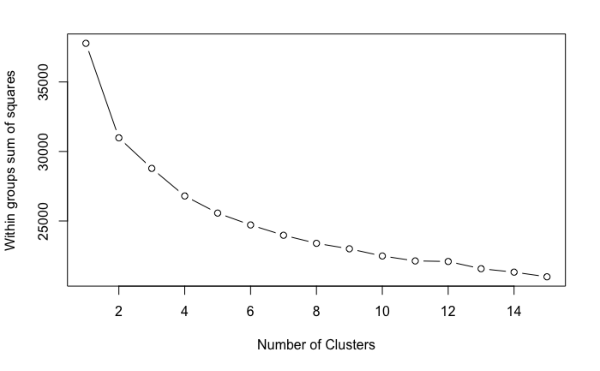
\includegraphics{Solo1_files/figure-latex/unnamed-chunk-7-1.pdf}

\subsection{\texorpdfstring{Imputing using
\texttt{mice}}{Imputing using mice}}\label{imputing-using-mice}

\begin{Shaded}
\begin{Highlighting}[]
\KeywordTok{map_df}\NormalTok{(df_nums,}\OperatorTok{~}\KeywordTok{as.factor}\NormalTok{(.x)) }\OperatorTok\StringTok{ }
\StringTok{  }\NormalTok{mice}\OperatorTok{::}\KeywordTok{mice}\NormalTok{(}\DataTypeTok{printFlag =}\NormalTok{ T, }\DataTypeTok{m =} \DecValTok{5}\NormalTok{, }\DataTypeTok{method =} \StringTok{'rf'}\NormalTok{) ->}\StringTok{ }\NormalTok{miceFit}
\end{Highlighting}
\end{Shaded}

\begin{verbatim}
## 
##  iter imp variable
##   1   1  q11  q57
##   1   2  q11  q57
##   1   3  q11  q57
##   1   4  q11  q57
##   1   5  q11  q57
##   2   1  q11  q57
##   2   2  q11  q57
##   2   3  q11  q57
##   2   4  q11  q57
##   2   5  q11  q57
##   3   1  q11  q57
##   3   2  q11  q57
##   3   3  q11  q57
##   3   4  q11  q57
##   3   5  q11  q57
##   4   1  q11  q57
##   4   2  q11  q57
##   4   3  q11  q57
##   4   4  q11  q57
##   4   5  q11  q57
##   5   1  q11  q57
##   5   2  q11  q57
##   5   3  q11  q57
##   5   4  q11  q57
##   5   5  q11  q57
\end{verbatim}

\begin{verbatim}
## Warning in as.POSIXlt.POSIXct(Sys.time()): unknown timezone 'default/
## America/Indiana/Indianapolis'
\end{verbatim}

\begin{verbatim}
## Warning: Number of logged events: 25
\end{verbatim}

\begin{Shaded}
\begin{Highlighting}[]
\NormalTok{df_nums <-}\StringTok{ }\KeywordTok{tbl_df}\NormalTok{(mice}\OperatorTok{::}\KeywordTok{complete}\NormalTok{(miceFit))}
\end{Highlighting}
\end{Shaded}

\section{Bi Plots}\label{bi-plots}

\begin{Shaded}
\begin{Highlighting}[]
\CommentTok{# questions_to_consolidate <- c('q13','q24','q25','q26')}
\CommentTok{# plot_bi_plots(df_nums %>% dplyr::select(contains(questions_to_consolidate[1])),questions_to_consolidate[1])}
\CommentTok{# plot_bi_plots(df_nums %>% dplyr::select(contains(questions_to_consolidate[2])),questions_to_consolidate[2], xlim=c(0,.05), ylim=c(-0.01,0.002))}
\CommentTok{# plot_bi_plots(df_nums %>% dplyr::select(contains(questions_to_consolidate[3])),questions_to_consolidate[3])}
\CommentTok{# plot_bi_plots(df_nums %>% dplyr::select(contains(questions_to_consolidate[4])),questions_to_consolidate[4], xlim=c(0,0.05),ylim=c(-0.011,0.005))}
\end{Highlighting}
\end{Shaded}

\section{Data Prep}\label{data-prep-1}

\subsection{Sub grouping}\label{sub-grouping}

\begin{Shaded}
\begin{Highlighting}[]
\NormalTok{df_nums <-}\StringTok{ }\KeywordTok{map_df}\NormalTok{(df_nums,}\OperatorTok{~}\KeywordTok{as.numeric}\NormalTok{(}\KeywordTok{as.character}\NormalTok{(.x)))}
\NormalTok{df_nums_adj <-}\StringTok{ }\NormalTok{df_nums }\OperatorTok\StringTok{  }
\StringTok{  }\KeywordTok{adjust_q13}\NormalTok{() }\OperatorTok\StringTok{ }
\StringTok{  }\KeywordTok{adjust_q24}\NormalTok{() }\OperatorTok\StringTok{ }
\StringTok{  }\KeywordTok{adjust_q25}\NormalTok{() }\OperatorTok\StringTok{ }
\StringTok{  }\KeywordTok{adjust_q26}\NormalTok{() }\OperatorTok\StringTok{ }
\StringTok{  }\KeywordTok{adjust_q2}\NormalTok{() }\OperatorTok\StringTok{ }
\StringTok{  }\KeywordTok{adjust_q4}\NormalTok{() }\OperatorTok\StringTok{ }
\StringTok{  }\KeywordTok{adjust_race}\NormalTok{() }\OperatorTok\StringTok{ }
\StringTok{  }\KeywordTok{adjust_gender}\NormalTok{() }\OperatorTok\StringTok{ }
\StringTok{  }\KeywordTok{adjust_marital}\NormalTok{() }\OperatorTok\StringTok{ }
\StringTok{  }\KeywordTok{adjust_income}\NormalTok{() }\OperatorTok
\StringTok{  }\KeywordTok{adjust_age}\NormalTok{() }\OperatorTok\StringTok{ }
\StringTok{  }\KeywordTok{adjust_q11}\NormalTok{() }\OperatorTok\StringTok{ }
\StringTok{  }\KeywordTok{adjust_names}\NormalTok{() }\OperatorTok\StringTok{ }
\StringTok{  }\KeywordTok{adjust_children}\NormalTok{()}
\end{Highlighting}
\end{Shaded}

\begin{verbatim}
## Warning: package 'bindrcpp' was built under R version 3.4.4
\end{verbatim}

\begin{Shaded}
\begin{Highlighting}[]
\KeywordTok{glimpse}\NormalTok{(df_nums_adj)}
\end{Highlighting}
\end{Shaded}

\begin{verbatim}
## Observations: 1,800
## Variables: 43
## $ q1_age                   <dbl> 1, 1, 3, 1, 2, 1, 2, 2, 2, 2, 2, 1, 1...
## $ q11_appnum               <dbl> 4, 3, 3, 4, 3, 4, 4, 3, 1, 2, 3, 2, 4...
## $ q12_freeapppc            <dbl> 5, 5, 6, 4, 6, 3, 3, 6, 5, 2, 5, 6, 2...
## $ q48_edu                  <dbl> 3, 4, 3, 4, 4, 1, 3, 4, 3, 3, 4, 3, 4...
## $ q49_marital              <dbl> 0, 0, 1, 0, 1, 0, 0, 0, 1, 1, 1, 0, 0...
## $ q50r1_nochild            <dbl> 1, 1, 0, 1, 0, 1, 0, 1, 0, 0, 1, 1, 1...
## $ q56_income               <dbl> 2, 3, 4, 2, 2, 1, 1, 3, 2, 2, 2, 2, 4...
## $ q57_mf                   <dbl> 1, 1, 1, 0, 1, 0, 0, 1, 0, 1, 1, 0, 0...
## $ q13_visitfreq_social     <dbl> 2.50, 3.00, 3.25, 4.00, 2.50, 4.00, 2...
## $ q13_visitfreq_music      <dbl> 3.75, 3.50, 2.75, 3.25, 3.50, 3.50, 4...
## $ q13_visitfreq_video      <dbl> 2.50, 2.00, 2.50, 2.50, 1.75, 2.25, 3...
## $ q24_tech_posatt          <dbl> 2.8, 2.8, 3.0, 3.0, 2.2, 3.4, 2.8, 2....
## $ q24_tech_enter           <dbl> 2.0, 2.0, 1.5, 3.0, 2.5, 1.0, 2.5, 2....
## $ q24_tech_comm            <dbl> 2.666667, 1.333333, 2.666667, 3.66666...
## $ q24_tech_negatv          <dbl> 1.0, 3.0, 4.5, 3.0, 1.5, 4.5, 1.5, 4....
## $ q25_prsnlty_leader       <dbl> 1.50, 2.75, 2.50, 2.00, 3.25, 3.00, 3...
## $ q25_prsnlty_risk         <dbl> 1.666667, 2.333333, 3.333333, 2.66666...
## $ q25_prsnlty_drive        <dbl> 2.75, 2.25, 2.00, 3.25, 3.00, 2.50, 2...
## $ q25_prsnlty_follower     <dbl> 5, 5, 6, 5, 4, 4, 2, 5, 5, 2, 6, 5, 2...
## $ q26_shopsavvy_bargain    <dbl> 2.5, 3.5, 3.0, 3.0, 3.0, 3.0, 3.5, 1....
## $ q26_shopsavvy_brands     <dbl> 3.4, 3.2, 3.4, 3.0, 4.0, 3.2, 2.8, 3....
## $ q26_shopsavvy_earn2spend <dbl> 2.666667, 3.333333, 3.666667, 3.66666...
## $ q26_shopsavvy_applover   <dbl> 4.166667, 3.000000, 4.166667, 2.16666...
## $ q26_shopsavvy_children   <dbl> 6, 6, 4, 6, 3, 5, 5, 6, 5, 1, 6, 6, 1...
## $ q2_apple                 <dbl> 0, 1, 0, 0, 1, 1, 1, 0, 0, 1, 1, 0, 1...
## $ q2_andriod               <dbl> 1, 0, 1, 1, 0, 0, 0, 0, 0, 0, 1, 0, 1...
## $ q2_windows               <dbl> 0, 0, 0, 0, 0, 0, 0, 0, 0, 0, 0, 0, 1...
## $ q2_tablet                <dbl> 0, 0, 0, 0, 1, 1, 0, 0, 0, 0, 0, 0, 1...
## $ q2_other                 <dbl> 0, 0, 0, 0, 1, 0, 0, 1, 1, 0, 0, 1, 1...
## $ q4_use_music_apps        <dbl> 1, 0, 0, 1, 1, 1, 1, 0, 0, 1, 0, 1, 1...
## $ q4_use_tv_apps           <dbl> 0, 0, 0, 0, 1, 1, 0, 0, 1, 1, 0, 0, 1...
## $ q4_use_game_apps         <dbl> 0, 1, 0, 1, 1, 1, 1, 1, 0, 0, 0, 1, 1...
## $ q4_use_social_apps       <dbl> 1, 1, 1, 1, 1, 0, 1, 1, 1, 0, 0, 1, 1...
## $ q4_use_news_apps         <dbl> 0, 0, 1, 0, 1, 0, 1, 1, 0, 1, 0, 0, 1...
## $ q4_use_shop_apps         <dbl> 0, 1, 1, 0, 1, 1, 0, 0, 0, 0, 0, 0, 1...
## $ q4_use_none_apps         <dbl> 0, 0, 0, 0, 0, 0, 0, 0, 0, 0, 0, 0, 0...
## $ q54_white                <dbl> 0, 1, 0, 1, 1, 1, 0, 1, 0, 1, 1, 1, 1...
## $ q54_black                <dbl> 0, 0, 1, 0, 0, 0, 1, 0, 0, 0, 0, 0, 0...
## $ q54_asian                <dbl> 0, 0, 0, 0, 0, 0, 0, 0, 0, 0, 0, 0, 0...
## $ q54_hawai                <dbl> 0, 0, 0, 0, 0, 0, 0, 0, 0, 0, 0, 0, 0...
## $ q54_native               <dbl> 0, 0, 0, 0, 0, 0, 0, 0, 0, 0, 0, 0, 0...
## $ q54_other                <dbl> 1, 0, 0, 0, 0, 0, 0, 0, 1, 0, 0, 0, 0...
## $ q55_latino               <dbl> 0, 0, 0, 0, 1, 0, 0, 0, 0, 0, 0, 0, 0...
\end{verbatim}

\subsection{Selection of basis
variables}\label{selection-of-basis-variables}

\begin{Shaded}
\begin{Highlighting}[]
\NormalTok{set1 <-}\StringTok{ }\KeywordTok{c}\NormalTok{(}
  \StringTok{'q1_age'}\NormalTok{,}
  \CommentTok{# 'q11_appnum',}
  \CommentTok{# 'q12_freeapppc',}
  \StringTok{'q48_edu'}\NormalTok{,}
  \StringTok{'q49_marital'}\NormalTok{,}
  \StringTok{'q50r1_nochild'}\NormalTok{,}
  \StringTok{'q56_income'}\NormalTok{,}
  \CommentTok{# 'q57_mf',}
  \CommentTok{# 'q13_visitfreq_social',}
  \CommentTok{# 'q13_visitfreq_music',}
  \CommentTok{# 'q13_visitfreq_video',}
  \StringTok{'q24_tech_posatt'}\NormalTok{,}
  \StringTok{'q24_tech_enter'}\NormalTok{,}
  \StringTok{'q24_tech_comm'}\NormalTok{,}
  \StringTok{'q24_tech_negatv'}\NormalTok{,}
  \CommentTok{# 'q25_prsnlty_leader',}
  \CommentTok{# 'q25_prsnlty_risk',}
  \CommentTok{# 'q25_prsnlty_drive',}
  \CommentTok{# 'q25_prsnlty_follower',}
  \StringTok{'q26_shopsavvy_bargain'}\NormalTok{,}
  \StringTok{'q26_shopsavvy_brands'}\NormalTok{,}
  \StringTok{'q26_shopsavvy_earn2spend'}\NormalTok{,}
  \StringTok{'q26_shopsavvy_applover'}\NormalTok{,}
  \StringTok{'q26_shopsavvy_children'}\NormalTok{,}
  \StringTok{'q2_apple'}\NormalTok{,}
  \StringTok{'q2_andriod'}\NormalTok{,}
  \StringTok{'q2_windows'}\NormalTok{,}
  \CommentTok{# 'q2_tablet',}
  \CommentTok{# 'q2_other',}
  \CommentTok{# 'q4_use_music_apps',}
  \CommentTok{# 'q4_use_tv_apps',}
  \CommentTok{# 'q4_use_game_apps',}
  \CommentTok{# 'q4_use_social_apps',}
  \CommentTok{# 'q4_use_news_apps',}
  \CommentTok{# 'q4_use_shop_apps',}
  \CommentTok{# 'q4_use_none_apps',}
  \StringTok{'q54_white'}\NormalTok{,}
  \StringTok{'q54_black'}\NormalTok{,}
  \StringTok{'q54_asian'}\NormalTok{,}
  \StringTok{'q54_hawai'}\NormalTok{,}
  \StringTok{'q54_native'}\NormalTok{,}
  \CommentTok{# 'q54_other',}
  \StringTok{'q55_latino'}
\NormalTok{  )}
\NormalTok{set2 <-}\StringTok{ }\KeywordTok{c}\NormalTok{(}
  \StringTok{'q1_age'}\NormalTok{,}
  \CommentTok{# 'q11_appnum',}
  \StringTok{'q12_freeapppc'}\NormalTok{,}
  \StringTok{'q48_edu'}\NormalTok{,}
  \StringTok{'q49_marital'}\NormalTok{,}
  \StringTok{'q50r1_nochild'}\NormalTok{,}
  \StringTok{'q56_income'}\NormalTok{,}
  \CommentTok{# 'q57_mf',}
  \StringTok{'q13_visitfreq_social'}\NormalTok{,}
  \StringTok{'q13_visitfreq_music'}\NormalTok{,}
  \StringTok{'q13_visitfreq_video'}\NormalTok{,}
  \StringTok{'q24_tech_posatt'}\NormalTok{,}
  \StringTok{'q24_tech_enter'}\NormalTok{,}
  \StringTok{'q24_tech_comm'}\NormalTok{,}
  \StringTok{'q24_tech_negatv'}\NormalTok{,}
  \StringTok{'q25_prsnlty_leader'}\NormalTok{,}
  \StringTok{'q25_prsnlty_risk'}\NormalTok{,}
  \StringTok{'q25_prsnlty_drive'}\NormalTok{,}
  \StringTok{'q25_prsnlty_follower'}\NormalTok{,}
  \StringTok{'q26_shopsavvy_bargain'}\NormalTok{,}
  \StringTok{'q26_shopsavvy_brands'}\NormalTok{,}
  \StringTok{'q26_shopsavvy_earn2spend'}\NormalTok{,}
  \StringTok{'q26_shopsavvy_applover'}\NormalTok{,}
  \StringTok{'q26_shopsavvy_children'}\NormalTok{,}
  \CommentTok{# 'q2_apple',}
  \CommentTok{# 'q2_andriod',}
  \CommentTok{# 'q2_windows',}
  \CommentTok{# 'q2_tablet',}
  \CommentTok{# 'q2_other',}
  \CommentTok{# 'q4_use_music_apps',}
  \CommentTok{# 'q4_use_tv_apps',}
  \CommentTok{# 'q4_use_game_apps',}
  \CommentTok{# 'q4_use_social_apps',}
  \CommentTok{# 'q4_use_news_apps',}
  \CommentTok{# 'q4_use_shop_apps',}
  \CommentTok{# 'q4_use_none_apps',}
  \StringTok{'q54_white'}\NormalTok{,}
  \StringTok{'q54_black'}\NormalTok{,}
  \StringTok{'q54_asian'}\NormalTok{,}
  \StringTok{'q54_hawai'}\NormalTok{,}
  \StringTok{'q54_native'}\NormalTok{,}
  \CommentTok{# 'q54_other',}
  \StringTok{'q55_latino'}
\NormalTok{  )}
\NormalTok{set3 <-}\StringTok{ }\KeywordTok{c}\NormalTok{(}
  \StringTok{'q1_age'}\NormalTok{,}
  \StringTok{'q11_appnum'}\NormalTok{,}
  \StringTok{'q12_freeapppc'}\NormalTok{,}
  \StringTok{'q48_edu'}\NormalTok{,}
  \StringTok{'q49_marital'}\NormalTok{,}
  \StringTok{'q50r1_nochild'}\NormalTok{,}
  \StringTok{'q56_income'}\NormalTok{,}
  \StringTok{'q57_mf'}\NormalTok{,}
  \CommentTok{# 'q13_visitfreq_social',}
  \CommentTok{# 'q13_visitfreq_music',}
  \CommentTok{# 'q13_visitfreq_video',}
  \CommentTok{# 'q24_tech_posatt',}
  \CommentTok{# 'q24_tech_enter',}
  \CommentTok{# 'q24_tech_comm',}
  \CommentTok{# 'q24_tech_negatv',}
  \CommentTok{# 'q25_prsnlty_leader',}
  \CommentTok{# 'q25_prsnlty_risk',}
  \CommentTok{# 'q25_prsnlty_drive',}
  \CommentTok{# 'q25_prsnlty_follower',}
  \StringTok{'q26_shopsavvy_bargain'}\NormalTok{,}
  \StringTok{'q26_shopsavvy_brands'}\NormalTok{,}
  \StringTok{'q26_shopsavvy_earn2spend'}\NormalTok{,}
  \StringTok{'q26_shopsavvy_applover'}\NormalTok{,}
  \StringTok{'q26_shopsavvy_children'}\NormalTok{,}
  \StringTok{'q2_apple'}\NormalTok{,}
  \StringTok{'q2_andriod'}\NormalTok{,}
  \StringTok{'q2_windows'}\NormalTok{,}
  \StringTok{'q2_tablet'}\NormalTok{,}
  \StringTok{'q2_other'}\NormalTok{,}
  \StringTok{'q4_use_music_apps'}\NormalTok{,}
  \StringTok{'q4_use_tv_apps'}\NormalTok{,}
  \StringTok{'q4_use_game_apps'}\NormalTok{,}
  \StringTok{'q4_use_social_apps'}\NormalTok{,}
  \StringTok{'q4_use_news_apps'}\NormalTok{,}
  \StringTok{'q4_use_shop_apps'}\NormalTok{,}
  \StringTok{'q4_use_none_apps'}
  \CommentTok{# 'q54_white',}
  \CommentTok{# 'q54_black',}
  \CommentTok{# 'q54_asian',}
  \CommentTok{# 'q54_hawai',}
  \CommentTok{# 'q54_native',}
  \CommentTok{# 'q54_other',}
  \CommentTok{# 'q55_latino'}
\NormalTok{  )}
\NormalTok{set4 <-}\StringTok{ }\KeywordTok{c}\NormalTok{(}
  \StringTok{'q1_age'}\NormalTok{,}
  \CommentTok{# 'q11_appnum',}
  \CommentTok{# 'q12_freeapppc',}
  \CommentTok{# 'q48_edu',}
  \StringTok{'q49_marital'}\NormalTok{,}
  \StringTok{'q50r1_nochild'}\NormalTok{,}
  \StringTok{'q56_income'}\NormalTok{,}
  \StringTok{'q57_mf'}\NormalTok{,}
  \StringTok{'q13_visitfreq_social'}\NormalTok{,}
  \StringTok{'q13_visitfreq_music'}\NormalTok{,}
  \StringTok{'q13_visitfreq_video'}\NormalTok{,}
  \StringTok{'q24_tech_posatt'}\NormalTok{,}
  \StringTok{'q24_tech_enter'}\NormalTok{,}
  \StringTok{'q24_tech_comm'}\NormalTok{,}
  \StringTok{'q24_tech_negatv'}\NormalTok{,}
  \StringTok{'q25_prsnlty_leader'}\NormalTok{,}
  \StringTok{'q25_prsnlty_risk'}\NormalTok{,}
  \StringTok{'q25_prsnlty_drive'}\NormalTok{,}
  \StringTok{'q25_prsnlty_follower'}\NormalTok{,}
  \StringTok{'q26_shopsavvy_bargain'}\NormalTok{,}
  \StringTok{'q26_shopsavvy_brands'}\NormalTok{,}
  \StringTok{'q26_shopsavvy_earn2spend'}\NormalTok{,}
  \StringTok{'q26_shopsavvy_applover'}\NormalTok{,}
  \StringTok{'q26_shopsavvy_children'}
  \CommentTok{# 'q2_apple',}
  \CommentTok{# 'q2_andriod',}
  \CommentTok{# 'q2_windows',}
  \CommentTok{# 'q2_tablet',}
  \CommentTok{# 'q2_other',}
  \CommentTok{# 'q4_use_music_apps',}
  \CommentTok{# 'q4_use_tv_apps',}
  \CommentTok{# 'q4_use_game_apps',}
  \CommentTok{# 'q4_use_social_apps',}
  \CommentTok{# 'q4_use_news_apps',}
  \CommentTok{# 'q4_use_shop_apps',}
  \CommentTok{# 'q4_use_none_apps'}
  \CommentTok{# 'q54_white',}
  \CommentTok{# 'q54_black',}
  \CommentTok{# 'q54_asian',}
  \CommentTok{# 'q54_hawai',}
  \CommentTok{# 'q54_native',}
  \CommentTok{# 'q54_other',}
  \CommentTok{# 'q55_latino'}
\NormalTok{  )}
\end{Highlighting}
\end{Shaded}

\begin{Shaded}
\begin{Highlighting}[]
\NormalTok{df_nums_adj_backup <-}\StringTok{ }\NormalTok{df_nums_adj}
\end{Highlighting}
\end{Shaded}

\begin{Shaded}
\begin{Highlighting}[]
\NormalTok{df_nums_adj <-}\StringTok{ }\NormalTok{df_nums_adj_backup}
\end{Highlighting}
\end{Shaded}

\begin{Shaded}
\begin{Highlighting}[]
\NormalTok{df_nums_adj <-}\StringTok{ }\NormalTok{df_nums_adj }\OperatorTok\StringTok{ }\NormalTok{dplyr}\OperatorTok{::}\KeywordTok{select}\NormalTok{(}\KeywordTok{one_of}\NormalTok{(set4))}
\end{Highlighting}
\end{Shaded}

\section{Scaling}\label{scaling}

\begin{Shaded}
\begin{Highlighting}[]
\NormalTok{scaling_wanted <-}\StringTok{ }\NormalTok{T}
\NormalTok{minmax_wanted <-}\StringTok{ }\NormalTok{F}
\ControlFlowTok{if}\NormalTok{ (scaling_wanted) \{}
\NormalTok{  df_nums_adjscaled <-}\StringTok{ }\KeywordTok{scale}\NormalTok{(df_nums_adj)}
\NormalTok{  centers <-}\StringTok{ }\KeywordTok{attributes}\NormalTok{(df_nums_adjscaled)[[}\DecValTok{3}\NormalTok{]]}
\NormalTok{  spreads <-}\StringTok{ }\KeywordTok{attributes}\NormalTok{(df_nums_adjscaled)[[}\DecValTok{4}\NormalTok{]]}
\NormalTok{  df_nums_adjscaled <-}\StringTok{ }\KeywordTok{tbl_df}\NormalTok{(df_nums_adjscaled)}
\NormalTok{\}}
\ControlFlowTok{if}\NormalTok{(minmax_wanted)\{}
\NormalTok{  df_nums_adjscaled <-}\StringTok{ }\KeywordTok{map_df}\NormalTok{(df_nums_adj, }\OperatorTok{~}\KeywordTok{minmax}\NormalTok{(.x))}
\NormalTok{\}}
\ControlFlowTok{if}\NormalTok{(}\OperatorTok{!}\NormalTok{scaling_wanted }\OperatorTok{&}\StringTok{ }\OperatorTok{!}\NormalTok{minmax_wanted)\{}
\NormalTok{  df_nums_adjscaled <-}\StringTok{ }\NormalTok{df_nums_adj}
\NormalTok{\}}
\KeywordTok{head}\NormalTok{(df_nums_adjscaled)}
\end{Highlighting}
\end{Shaded}

\begin{verbatim}
## # A tibble: 6 x 21
##   q1_age q49_marital q50r1_nochild q56_income q57_mf q13_visitfreq_social
##    <dbl>       <dbl>         <dbl>      <dbl>  <dbl>                <dbl>
## 1 -1.28       -0.840         0.986     -0.458  1.05                -0.211
## 2 -1.28       -0.840         0.986      0.359  1.05                 0.496
## 3  0.945       1.19         -1.01       1.18   1.05                 0.849
## 4 -1.28       -0.840         0.986     -0.458 -0.955                1.91 
## 5 -0.167       1.19         -1.01      -0.458  1.05                -0.211
## 6 -1.28       -0.840         0.986     -1.27  -0.955                1.91 
## # ... with 15 more variables: q13_visitfreq_music <dbl>,
## #   q13_visitfreq_video <dbl>, q24_tech_posatt <dbl>,
## #   q24_tech_enter <dbl>, q24_tech_comm <dbl>, q24_tech_negatv <dbl>,
## #   q25_prsnlty_leader <dbl>, q25_prsnlty_risk <dbl>,
## #   q25_prsnlty_drive <dbl>, q25_prsnlty_follower <dbl>,
## #   q26_shopsavvy_bargain <dbl>, q26_shopsavvy_brands <dbl>,
## #   q26_shopsavvy_earn2spend <dbl>, q26_shopsavvy_applover <dbl>,
## #   q26_shopsavvy_children <dbl>
\end{verbatim}

\section{Correlation Plot}\label{correlation-plot}

\begin{Shaded}
\begin{Highlighting}[]
\NormalTok{df_nums_adjscaled }\OperatorTok\StringTok{ }\KeywordTok{cor}\NormalTok{() }\OperatorTok\StringTok{ }\KeywordTok{corrplot}\NormalTok{(}\DataTypeTok{method =} \StringTok{'shade'}\NormalTok{,}\DataTypeTok{tl.col =} \StringTok{'black'}\NormalTok{,}\DataTypeTok{tl.cex =}\NormalTok{ .}\DecValTok{9}\NormalTok{, }\DataTypeTok{order =} \StringTok{'hclust'}\NormalTok{, }\DataTypeTok{hclust.method =} \StringTok{'ward.D2'}\NormalTok{)}
\end{Highlighting}
\end{Shaded}

\includegraphics{Solo1_files/figure-latex/unnamed-chunk-16-1.pdf}

\section{Dissimilarity Calculations}\label{dissimilarity-calculations}

\begin{Shaded}
\begin{Highlighting}[]
\CommentTok{# ordered=c(1:4,11,13:28)}
\CommentTok{# symm_bin=c(6:10,12,29:47)}
\CommentTok{# df_nums_adjscaled[ordered] <- map_df(df_nums_adjscaled[ordered],~as.ordered(.x))}
\CommentTok{# df_nums_adjscaled[symm_bin] <- map_df(df_nums_adjscaled[symm_bin],~as.factor(.x))}
\NormalTok{distMat <-}\StringTok{ }\KeywordTok{daisy}\NormalTok{(df_nums_adjscaled)}
\end{Highlighting}
\end{Shaded}

\begin{verbatim}
## Warning in daisy(df_nums_adjscaled): binary variable(s) 2, 3, 5 treated as
## interval scaled
\end{verbatim}

\section{Simple clustering}\label{simple-clustering}

\subsection{H clust}\label{h-clust}

\subsubsection{How cophenetic changes with clustering
method?}\label{how-cophenetic-changes-with-clustering-method}

\begin{Shaded}
\begin{Highlighting}[]
\NormalTok{methods <-}\StringTok{ }\KeywordTok{c}\NormalTok{(}\StringTok{'complete'}\NormalTok{,}\StringTok{'average'}\NormalTok{,}\StringTok{'ward.D'}\NormalTok{,}\StringTok{'ward.D2'}\NormalTok{,}\StringTok{'median'}\NormalTok{,}\StringTok{'mcquitty'}\NormalTok{,}\StringTok{'centroid'}\NormalTok{)}
\NormalTok{method_vs_cop <-}\StringTok{ }\KeywordTok{map_dbl}\NormalTok{(methods,}\OperatorTok{~}\KeywordTok{cor}\NormalTok{(}\KeywordTok{cophenetic}\NormalTok{(}\KeywordTok{hclust}\NormalTok{(}\DataTypeTok{d =}\NormalTok{ distMat, }\DataTypeTok{method =}\NormalTok{ .x)), distMat))}
\KeywordTok{names}\NormalTok{(method_vs_cop) <-}\StringTok{ }\NormalTok{methods}
\KeywordTok{barchart}\NormalTok{(}\KeywordTok{sort}\NormalTok{(method_vs_cop))}
\end{Highlighting}
\end{Shaded}

\includegraphics{Solo1_files/figure-latex/unnamed-chunk-18-1.pdf}

\begin{Shaded}
\begin{Highlighting}[]
\NormalTok{k =}\StringTok{ }\DecValTok{6}
\NormalTok{hclustFit <-}\StringTok{ }\KeywordTok{hclust}\NormalTok{(}\DataTypeTok{d =}\NormalTok{ distMat, }\DataTypeTok{method =} \StringTok{'ward.D'}\NormalTok{)}
\KeywordTok{plot}\NormalTok{(hclustFit, }\DataTypeTok{labels =}\NormalTok{ F)}
\KeywordTok{rect.hclust}\NormalTok{(hclustFit, }\DataTypeTok{k=}\NormalTok{k, }\DataTypeTok{border=}\StringTok{"red"}\NormalTok{)}
\end{Highlighting}
\end{Shaded}

\includegraphics{Solo1_files/figure-latex/unnamed-chunk-19-1.pdf}

\begin{Shaded}
\begin{Highlighting}[]
\NormalTok{hclust_segments <-}\StringTok{ }\KeywordTok{cutree}\NormalTok{(hclustFit, }\DataTypeTok{k =}\NormalTok{ k)}
\KeywordTok{table}\NormalTok{(hclust_segments)}
\end{Highlighting}
\end{Shaded}

\begin{verbatim}
## hclust_segments
##   1   2   3   4   5   6 
## 495 495 165 135 151 359
\end{verbatim}

\begin{Shaded}
\begin{Highlighting}[]
\KeywordTok{clusplot}\NormalTok{(df_nums_adjscaled, hclust_segments, }\DataTypeTok{color=}\OtherTok{TRUE}\NormalTok{, }\DataTypeTok{shade=}\OtherTok{TRUE}\NormalTok{, }\DataTypeTok{labels=}\DecValTok{4}\NormalTok{, }\DataTypeTok{lines=}\DecValTok{0}\NormalTok{, }\DataTypeTok{main=}\StringTok{"HClust plot"}\NormalTok{)}
\end{Highlighting}
\end{Shaded}

\includegraphics{Solo1_files/figure-latex/unnamed-chunk-20-1.pdf}

\begin{Shaded}
\begin{Highlighting}[]
\KeywordTok{seg.summ}\NormalTok{(df_nums_adj, hclust_segments) ->}\StringTok{ }\NormalTok{centroids}
\NormalTok{centroids}
\end{Highlighting}
\end{Shaded}

\begin{verbatim}
##   Group.1   q1_age q49_marital q50r1_nochild q56_income    q57_mf
## 1       1 1.896970   0.2181818    0.94343434   2.494949 0.3878788
## 2       2 2.620202   0.6383838    0.08888889   2.870707 0.5959596
## 3       3 1.460606   0.1090909    0.75757576   1.903030 0.3090909
## 4       4 1.844444   0.5185185    0.37037037   2.614815 0.3703704
## 5       5 3.066225   0.6026490    0.33774834   2.947020 0.6821192
## 6       6 1.899721   0.3955432    0.48746518   2.342618 0.4679666
##   q13_visitfreq_social q13_visitfreq_music q13_visitfreq_video
## 1             2.746970            3.234343            2.489394
## 2             2.790404            3.253535            2.792929
## 3             2.727273            3.021212            2.577273
## 4             1.533333            1.757407            1.537037
## 5             3.394040            3.597682            3.248344
## 6             2.389276            2.698468            2.252786
##   q24_tech_posatt q24_tech_enter q24_tech_comm q24_tech_negatv
## 1        2.287677       1.805051      1.913131        3.927273
## 2        2.494141       2.045455      2.272054        3.690909
## 3        3.010909       3.193939      3.258586        3.230303
## 4        1.678519       1.670370      1.649383        1.988889
## 5        3.323179       3.066225      3.328918        3.645695
## 6        1.841783       1.525070      1.595172        3.454039
##   q25_prsnlty_leader q25_prsnlty_risk q25_prsnlty_drive
## 1           2.342929         2.370370          2.468687
## 2           2.472727         2.537374          2.397980
## 3           3.121212         3.141414          3.212121
## 4           1.572222         1.619753          1.612963
## 5           3.311258         3.346578          3.066225
## 6           1.695682         1.772516          1.885794
##   q25_prsnlty_follower q26_shopsavvy_bargain q26_shopsavvy_brands
## 1             4.727273              2.709091             3.307879
## 2             4.854545              2.730303             3.388283
## 3             3.581818              3.378788             3.676364
## 4             1.851852              1.692593             1.731852
## 5             4.993377              3.284768             4.211921
## 6             4.097493              2.019499             2.210585
##   q26_shopsavvy_earn2spend q26_shopsavvy_applover q26_shopsavvy_children
## 1                 3.381818               3.045791               5.298990
## 2                 3.531987               3.228956               3.391919
## 3                 3.701010               3.502020               4.060606
## 4                 1.738272               1.733333               1.725926
## 5                 4.187638               4.206402               4.715232
## 6                 2.289694               2.026927               3.150418
\end{verbatim}

\begin{Shaded}
\begin{Highlighting}[]
\NormalTok{cutFit <-}\StringTok{ }\KeywordTok{cutree}\NormalTok{(hclustFit, k)}
\KeywordTok{plot}\NormalTok{(}\KeywordTok{silhouette}\NormalTok{(cutFit,distMat))}
\end{Highlighting}
\end{Shaded}

\includegraphics{Solo1_files/figure-latex/unnamed-chunk-22-1.pdf}

\begin{Shaded}
\begin{Highlighting}[]
\NormalTok{k <-}\StringTok{ }\DecValTok{2}\OperatorTok{:}\DecValTok{10}
\NormalTok{widths <-}\StringTok{ }\OtherTok{NULL}
\ControlFlowTok{for}\NormalTok{(k_ }\ControlFlowTok{in}\NormalTok{ k)\{}
\NormalTok{  hclustFit <-}\StringTok{ }\KeywordTok{hclust}\NormalTok{(}\DataTypeTok{d =}\NormalTok{ distMat, }\DataTypeTok{method =} \StringTok{'ward.D'}\NormalTok{)}
\NormalTok{  cutFit <-}\StringTok{ }\KeywordTok{cutree}\NormalTok{(hclustFit, k_)}
\NormalTok{  widths <-}\StringTok{ }\KeywordTok{c}\NormalTok{(widths,}\KeywordTok{mean}\NormalTok{(}\KeywordTok{silhouette}\NormalTok{(cutFit,distMat)[,}\StringTok{'sil_width'}\NormalTok{]))}
\NormalTok{\}}
\KeywordTok{plot}\NormalTok{(k,widths,}\DataTypeTok{type=}\StringTok{'b'}\NormalTok{)}
\end{Highlighting}
\end{Shaded}

\includegraphics{Solo1_files/figure-latex/unnamed-chunk-23-1.pdf}

\begin{Shaded}
\begin{Highlighting}[]
\KeywordTok{cbind}\NormalTok{(k,widths)}
\end{Highlighting}
\end{Shaded}

\begin{verbatim}
##        k     widths
##  [1,]  2 0.14768060
##  [2,]  3 0.07761762
##  [3,]  4 0.07561574
##  [4,]  5 0.05913686
##  [5,]  6 0.05764810
##  [6,]  7 0.05370615
##  [7,]  8 0.04944634
##  [8,]  9 0.04325993
##  [9,] 10 0.04623427
\end{verbatim}

\subsection{K-means}\label{k-means}

\subsubsection{How many clusters to
use?}\label{how-many-clusters-to-use}

\begin{Shaded}
\begin{Highlighting}[]
\NormalTok{wssplot <-}\StringTok{ }\ControlFlowTok{function}\NormalTok{(numsub, }\DataTypeTok{nc=}\DecValTok{15}\NormalTok{, }\DataTypeTok{seed=}\DecValTok{1111}\NormalTok{) \{}
\NormalTok{  wss <-}\StringTok{ }\NormalTok{(}\KeywordTok{nrow}\NormalTok{(numsub)}\OperatorTok{-}\DecValTok{1}\NormalTok{)}\OperatorTok{*}\KeywordTok{sum}\NormalTok{(}\KeywordTok{apply}\NormalTok{(numsub,}\DecValTok{2}\NormalTok{,var))}
  \ControlFlowTok{for}\NormalTok{ (i }\ControlFlowTok{in} \DecValTok{2}\OperatorTok{:}\NormalTok{nc) \{}
    \KeywordTok{set.seed}\NormalTok{(seed)}
\NormalTok{    wss[i] <-}\StringTok{ }\KeywordTok{sum}\NormalTok{(}\KeywordTok{kmeans}\NormalTok{(numsub, }\DataTypeTok{centers=}\NormalTok{i, }\DataTypeTok{iter.max =} \FloatTok{1e4}\NormalTok{)}\OperatorTok{$}\NormalTok{withinss)\}}
  \KeywordTok{plot}\NormalTok{(}\DecValTok{1}\OperatorTok{:}\NormalTok{nc, wss, }\DataTypeTok{type=}\StringTok{"b"}\NormalTok{, }\DataTypeTok{xlab=}\StringTok{"Number of Clusters"}\NormalTok{,}
       \DataTypeTok{ylab=}\StringTok{"Within groups sum of squares"}\NormalTok{)\}}
\KeywordTok{wssplot}\NormalTok{(df_nums_adjscaled)}
\end{Highlighting}
\end{Shaded}

\includegraphics{Solo1_files/figure-latex/unnamed-chunk-24-1.pdf}

\subsubsection{Solving the k-means
model}\label{solving-the-k-means-model}

\begin{Shaded}
\begin{Highlighting}[]
\NormalTok{k <-}\StringTok{ }\DecValTok{2}\OperatorTok{:}\DecValTok{10}
\NormalTok{widths <-}\StringTok{ }\OtherTok{NULL}
\ControlFlowTok{for}\NormalTok{(k_ }\ControlFlowTok{in}\NormalTok{ k)\{}
\NormalTok{  clusterresults <-}\StringTok{ }\KeywordTok{kmeans}\NormalTok{(}\DataTypeTok{x =}\NormalTok{ df_nums_adjscaled, }\DataTypeTok{centers =}\NormalTok{ k_, }\DataTypeTok{nstart =} \DecValTok{30}\NormalTok{)}
\NormalTok{  widths <-}\StringTok{ }\KeywordTok{c}\NormalTok{(widths,}\KeywordTok{mean}\NormalTok{(}\KeywordTok{silhouette}\NormalTok{(clusterresults}\OperatorTok{$}\NormalTok{cluster,distMat)[,}\StringTok{'sil_width'}\NormalTok{]))}
\NormalTok{\}}
\KeywordTok{plot}\NormalTok{(k,widths,}\DataTypeTok{type=}\StringTok{'b'}\NormalTok{)}
\end{Highlighting}
\end{Shaded}

\includegraphics{Solo1_files/figure-latex/unnamed-chunk-25-1.pdf}

\begin{Shaded}
\begin{Highlighting}[]
\KeywordTok{cbind}\NormalTok{(k,widths)}
\end{Highlighting}
\end{Shaded}

\begin{verbatim}
##        k     widths
##  [1,]  2 0.15621386
##  [2,]  3 0.10957824
##  [3,]  4 0.10572588
##  [4,]  5 0.10283597
##  [5,]  6 0.09512150
##  [6,]  7 0.09265860
##  [7,]  8 0.08750201
##  [8,]  9 0.08336055
##  [9,] 10 0.08201107
\end{verbatim}

\begin{Shaded}
\begin{Highlighting}[]
\CommentTok{# Using cluster centers from hclust:}
\KeywordTok{seg.summ}\NormalTok{(df_nums_adjscaled, hclust_segments) ->}\StringTok{ }\NormalTok{kmeans_centroids}
\NormalTok{clusterresults <-}\StringTok{ }\KeywordTok{kmeans}\NormalTok{(}\DataTypeTok{x =}\NormalTok{ df_nums_adjscaled, }\DataTypeTok{centers =}\NormalTok{ kmeans_centroids[,}\OperatorTok{-}\DecValTok{1}\NormalTok{])}
\NormalTok{rsquare <-}\StringTok{ }\NormalTok{clusterresults}\OperatorTok{$}\NormalTok{betweenss}\OperatorTok{/}\NormalTok{clusterresults}\OperatorTok{$}\NormalTok{totss}
\KeywordTok{cat}\NormalTok{(}\StringTok{'}\CharTok{\textbackslash{}n}\StringTok{Within SS:'}\NormalTok{,clusterresults}\OperatorTok{$}\NormalTok{withinss,}\StringTok{' Sizes:}\CharTok{\textbackslash{}n}\StringTok{'}\NormalTok{,clusterresults}\OperatorTok{$}\NormalTok{size,}\StringTok{'}\CharTok{\textbackslash{}n}\StringTok{rsq:'}\NormalTok{, rsquare)}
\end{Highlighting}
\end{Shaded}

\begin{verbatim}
## 
## Within SS: 4930.83 4855.729 3500.787 3110.679 3924.958 4351.218  Sizes:
##  383 374 257 236 235 315 
## rsq: 0.3468805
\end{verbatim}

\begin{Shaded}
\begin{Highlighting}[]
\KeywordTok{clusplot}\NormalTok{(df_nums_adjscaled, clusterresults}\OperatorTok{$}\NormalTok{cluster, }\DataTypeTok{color=}\OtherTok{TRUE}\NormalTok{, }\DataTypeTok{shade=}\OtherTok{TRUE}\NormalTok{, }\DataTypeTok{labels=}\DecValTok{4}\NormalTok{, }\DataTypeTok{lines=}\DecValTok{0}\NormalTok{, }\DataTypeTok{main=}\StringTok{"K-means cluster plot"}\NormalTok{)}
\end{Highlighting}
\end{Shaded}

\includegraphics{Solo1_files/figure-latex/unnamed-chunk-26-1.pdf}

\begin{Shaded}
\begin{Highlighting}[]
\KeywordTok{plot}\NormalTok{(}\KeywordTok{silhouette}\NormalTok{(clusterresults}\OperatorTok{$}\NormalTok{cluster,distMat))}
\end{Highlighting}
\end{Shaded}

\includegraphics{Solo1_files/figure-latex/unnamed-chunk-26-2.pdf}

\begin{Shaded}
\begin{Highlighting}[]
\CommentTok{# Using number of clusters + random starts}
\NormalTok{k_kmeans =}\StringTok{ }\DecValTok{6}
\NormalTok{clusterresults <-}\StringTok{ }\KeywordTok{kmeans}\NormalTok{(}\DataTypeTok{x =}\NormalTok{ df_nums_adjscaled, }\DataTypeTok{centers =}\NormalTok{ k_kmeans)}
\NormalTok{rsquare <-}\StringTok{ }\NormalTok{clusterresults}\OperatorTok{$}\NormalTok{betweenss}\OperatorTok{/}\NormalTok{clusterresults}\OperatorTok{$}\NormalTok{totss}
\KeywordTok{cat}\NormalTok{(}\StringTok{'}\CharTok{\textbackslash{}n}\StringTok{Within SS:'}\NormalTok{,clusterresults}\OperatorTok{$}\NormalTok{withinss,}\StringTok{' Sizes:}\CharTok{\textbackslash{}n}\StringTok{'}\NormalTok{,clusterresults}\OperatorTok{$}\NormalTok{size,}\StringTok{'}\CharTok{\textbackslash{}n}\StringTok{rsq:'}\NormalTok{, rsquare)}
\end{Highlighting}
\end{Shaded}

\begin{verbatim}
## 
## Within SS: 4065.991 2967.302 5010.264 3974.676 4680.949 4116.096  Sizes:
##  315 227 377 295 321 265 
## rsq: 0.3431462
\end{verbatim}

\begin{Shaded}
\begin{Highlighting}[]
\KeywordTok{clusplot}\NormalTok{(df_nums_adjscaled, clusterresults}\OperatorTok{$}\NormalTok{cluster, }\DataTypeTok{color=}\OtherTok{TRUE}\NormalTok{, }\DataTypeTok{shade=}\OtherTok{TRUE}\NormalTok{, }\DataTypeTok{labels=}\DecValTok{4}\NormalTok{, }\DataTypeTok{lines=}\DecValTok{0}\NormalTok{, }\DataTypeTok{main=}\StringTok{"K-means cluster plot"}\NormalTok{)}
\end{Highlighting}
\end{Shaded}

\includegraphics{Solo1_files/figure-latex/unnamed-chunk-26-3.pdf}

\begin{Shaded}
\begin{Highlighting}[]
\KeywordTok{plot}\NormalTok{(}\KeywordTok{silhouette}\NormalTok{(clusterresults}\OperatorTok{$}\NormalTok{cluster,distMat))}
\end{Highlighting}
\end{Shaded}

\includegraphics{Solo1_files/figure-latex/unnamed-chunk-26-4.pdf}

\begin{Shaded}
\begin{Highlighting}[]
\KeywordTok{seg.summ}\NormalTok{(df_nums_adj, clusterresults}\OperatorTok{$}\NormalTok{cluster) ->}\StringTok{ }\NormalTok{segsummary_results}
\NormalTok{segsummary_results }\OperatorTok\StringTok{ }\KeywordTok{write_csv}\NormalTok{(}\DataTypeTok{path =} \StringTok{'../reports/kmeans_results.csv'}\NormalTok{, }\DataTypeTok{col_names =}\NormalTok{ T)}
\NormalTok{segsummary_results}
\end{Highlighting}
\end{Shaded}

\begin{verbatim}
##   Group.1   q1_age q49_marital q50r1_nochild q56_income    q57_mf
## 1       1 1.977778   0.1777778     0.9174603   2.425397 0.3777778
## 2       2 1.819383   0.4052863     0.4493392   2.431718 0.4052863
## 3       3 2.602122   0.7692308     0.0663130   3.015915 0.5358090
## 4       4 1.637288   0.1254237     0.8711864   2.257627 0.4576271
## 5       5 3.006231   0.7507788     0.1588785   3.021807 0.6479751
## 6       6 1.532075   0.1094340     0.7094340   1.962264 0.3886792
##   q13_visitfreq_social q13_visitfreq_music q13_visitfreq_video
## 1             2.853175            3.353968            2.604762
## 2             1.785242            1.991189            1.810573
## 3             2.575597            3.099469            2.548408
## 4             2.588983            2.972881            2.280508
## 5             3.191589            3.492991            3.171340
## 6             2.660377            2.958491            2.504717
##   q24_tech_posatt q24_tech_enter q24_tech_comm q24_tech_negatv
## 1        2.462222       1.804762      1.946032        4.160317
## 2        1.642291       1.599119      1.613803        2.158590
## 3        2.135809       1.567639      1.726790        4.145889
## 4        1.972203       1.601695      1.666667        3.566102
## 5        2.940810       2.710280      2.982347        3.353583
## 6        2.920755       3.033962      3.124528        3.286792
##   q25_prsnlty_leader q25_prsnlty_risk q25_prsnlty_drive
## 1           2.400794         2.387302          2.567460
## 2           1.580396         1.660793          1.645374
## 3           2.049072         2.109637          2.094164
## 4           1.759322         1.875706          2.022881
## 5           3.038941         3.101765          2.780374
## 6           3.161321         3.149686          3.153774
##   q25_prsnlty_follower q26_shopsavvy_bargain q26_shopsavvy_brands
## 1             5.047619              2.979365             3.774603
## 2             2.215859              1.669604             1.742731
## 3             5.050398              2.489390             2.982493
## 4             4.450847              2.138983             2.353898
## 5             4.897196              3.012461             3.943302
## 6             3.498113              3.190566             3.454340
##   q26_shopsavvy_earn2spend q26_shopsavvy_applover q26_shopsavvy_children
## 1                 3.886772               3.361376               5.495238
## 2                 1.741557               1.688693               1.797357
## 3                 3.176835               2.693634               3.071618
## 4                 2.457627               2.288136               4.684746
## 5                 3.979232               3.871236               4.084112
## 6                 3.405031               3.416352               3.992453
\end{verbatim}

\begin{Shaded}
\begin{Highlighting}[]
\NormalTok{kmeans_results <-}\StringTok{ }\NormalTok{df_nums_adj }\OperatorTok\StringTok{ }
\StringTok{  }\KeywordTok{mutate}\NormalTok{(}\DataTypeTok{cluster =}\NormalTok{ clusterresults}\OperatorTok{$}\NormalTok{cluster)}

\NormalTok{purrr}\OperatorTok{::}\KeywordTok{map2}\NormalTok{(kmeans_results, }\KeywordTok{names}\NormalTok{(kmeans_results),}
            \OperatorTok{~}\KeywordTok{bwplot}\NormalTok{(cluster}\OperatorTok{~}\NormalTok{.x, kmeans_results,}
                    \DataTypeTok{main=}\NormalTok{.y))}
\end{Highlighting}
\end{Shaded}

\begin{verbatim}
## $q1_age
\end{verbatim}

\includegraphics{Solo1_files/figure-latex/unnamed-chunk-28-1.pdf}

\begin{verbatim}
## 
## $q49_marital
\end{verbatim}

\includegraphics{Solo1_files/figure-latex/unnamed-chunk-28-2.pdf}

\begin{verbatim}
## 
## $q50r1_nochild
\end{verbatim}

\includegraphics{Solo1_files/figure-latex/unnamed-chunk-28-3.pdf}

\begin{verbatim}
## 
## $q56_income
\end{verbatim}

\includegraphics{Solo1_files/figure-latex/unnamed-chunk-28-4.pdf}

\begin{verbatim}
## 
## $q57_mf
\end{verbatim}

\includegraphics{Solo1_files/figure-latex/unnamed-chunk-28-5.pdf}

\begin{verbatim}
## 
## $q13_visitfreq_social
\end{verbatim}

\includegraphics{Solo1_files/figure-latex/unnamed-chunk-28-6.pdf}

\begin{verbatim}
## 
## $q13_visitfreq_music
\end{verbatim}

\includegraphics{Solo1_files/figure-latex/unnamed-chunk-28-7.pdf}

\begin{verbatim}
## 
## $q13_visitfreq_video
\end{verbatim}

\includegraphics{Solo1_files/figure-latex/unnamed-chunk-28-8.pdf}

\begin{verbatim}
## 
## $q24_tech_posatt
\end{verbatim}

\includegraphics{Solo1_files/figure-latex/unnamed-chunk-28-9.pdf}

\begin{verbatim}
## 
## $q24_tech_enter
\end{verbatim}

\includegraphics{Solo1_files/figure-latex/unnamed-chunk-28-10.pdf}

\begin{verbatim}
## 
## $q24_tech_comm
\end{verbatim}

\includegraphics{Solo1_files/figure-latex/unnamed-chunk-28-11.pdf}

\begin{verbatim}
## 
## $q24_tech_negatv
\end{verbatim}

\includegraphics{Solo1_files/figure-latex/unnamed-chunk-28-12.pdf}

\begin{verbatim}
## 
## $q25_prsnlty_leader
\end{verbatim}

\includegraphics{Solo1_files/figure-latex/unnamed-chunk-28-13.pdf}

\begin{verbatim}
## 
## $q25_prsnlty_risk
\end{verbatim}

\includegraphics{Solo1_files/figure-latex/unnamed-chunk-28-14.pdf}

\begin{verbatim}
## 
## $q25_prsnlty_drive
\end{verbatim}

\includegraphics{Solo1_files/figure-latex/unnamed-chunk-28-15.pdf}

\begin{verbatim}
## 
## $q25_prsnlty_follower
\end{verbatim}

\includegraphics{Solo1_files/figure-latex/unnamed-chunk-28-16.pdf}

\begin{verbatim}
## 
## $q26_shopsavvy_bargain
\end{verbatim}

\includegraphics{Solo1_files/figure-latex/unnamed-chunk-28-17.pdf}

\begin{verbatim}
## 
## $q26_shopsavvy_brands
\end{verbatim}

\includegraphics{Solo1_files/figure-latex/unnamed-chunk-28-18.pdf}

\begin{verbatim}
## 
## $q26_shopsavvy_earn2spend
\end{verbatim}

\includegraphics{Solo1_files/figure-latex/unnamed-chunk-28-19.pdf}

\begin{verbatim}
## 
## $q26_shopsavvy_applover
\end{verbatim}

\includegraphics{Solo1_files/figure-latex/unnamed-chunk-28-20.pdf}

\begin{verbatim}
## 
## $q26_shopsavvy_children
\end{verbatim}

\includegraphics{Solo1_files/figure-latex/unnamed-chunk-28-21.pdf}

\begin{verbatim}
## 
## $cluster
\end{verbatim}

\includegraphics{Solo1_files/figure-latex/unnamed-chunk-28-22.pdf}

\subsection{PAM}\label{pam}

\begin{Shaded}
\begin{Highlighting}[]
\NormalTok{pamFits <-}\StringTok{ }\KeywordTok{tibble}\NormalTok{(}\DataTypeTok{k_pam =} \DecValTok{2}\OperatorTok{:}\DecValTok{10}\NormalTok{)}
\NormalTok{pamFits}\OperatorTok{$}\NormalTok{pamFits <-}\StringTok{ }\KeywordTok{map}\NormalTok{(pamFits}\OperatorTok{$}\NormalTok{k_pam, }\OperatorTok{~}\KeywordTok{pam}\NormalTok{(df_nums_adjscaled, }\DataTypeTok{k =}\NormalTok{ .x))}
\NormalTok{pamFits}\OperatorTok{$}\NormalTok{sil_avg_width <-}\StringTok{ }\KeywordTok{map_dbl}\NormalTok{(pamFits}\OperatorTok{$}\NormalTok{pamFits,}\OperatorTok{~}\NormalTok{.x}\OperatorTok{$}\NormalTok{silinfo}\OperatorTok{$}\NormalTok{avg.width)}
\NormalTok{pamFits}
\end{Highlighting}
\end{Shaded}

\begin{verbatim}
## # A tibble: 9 x 3
##   k_pam pamFits   sil_avg_width
##   <int> <list>            <dbl>
## 1     2 <S3: pam>        0.136 
## 2     3 <S3: pam>        0.0961
## 3     4 <S3: pam>        0.0849
## 4     5 <S3: pam>        0.0731
## 5     6 <S3: pam>        0.0740
## 6     7 <S3: pam>        0.0680
## 7     8 <S3: pam>        0.0639
## 8     9 <S3: pam>        0.0651
## 9    10 <S3: pam>        0.0625
\end{verbatim}

\begin{Shaded}
\begin{Highlighting}[]
\NormalTok{pamFits }\OperatorTok\StringTok{ }
\StringTok{  }\KeywordTok{xyplot}\NormalTok{(sil_avg_width}\OperatorTok{~}\KeywordTok{as.factor}\NormalTok{(k_pam),.,}\DataTypeTok{type=}\StringTok{'b'}\NormalTok{)}
\end{Highlighting}
\end{Shaded}

\includegraphics{Solo1_files/figure-latex/unnamed-chunk-30-1.pdf}

\begin{Shaded}
\begin{Highlighting}[]
\KeywordTok{plot}\NormalTok{(pamFits}\OperatorTok{$}\NormalTok{pamFits[[}\DecValTok{1}\NormalTok{]])}
\end{Highlighting}
\end{Shaded}

\includegraphics{Solo1_files/figure-latex/unnamed-chunk-31-1.pdf}
\includegraphics{Solo1_files/figure-latex/unnamed-chunk-31-2.pdf}

\begin{Shaded}
\begin{Highlighting}[]
\KeywordTok{seg.summ}\NormalTok{(df_nums_adj, pamFits}\OperatorTok{$}\NormalTok{pamFits[[}\DecValTok{1}\NormalTok{]]}\OperatorTok{$}\NormalTok{clustering)}
\end{Highlighting}
\end{Shaded}

\begin{verbatim}
##   Group.1   q1_age q49_marital q50r1_nochild q56_income    q57_mf
## 1       1 2.387772   0.5134003     0.4162479   2.690117 0.5452261
## 2       2 1.683168   0.2178218     0.6848185   2.305281 0.3432343
##   q13_visitfreq_social q13_visitfreq_music q13_visitfreq_video
## 1             2.823492            3.244975            2.746859
## 2             2.305281            2.615099            2.090759
##   q24_tech_posatt q24_tech_enter q24_tech_comm q24_tech_negatv
## 1        2.614238       2.268844      2.462032        3.675461
## 2        1.867987       1.584158      1.596810        3.258251
##   q25_prsnlty_leader q25_prsnlty_risk q25_prsnlty_drive
## 1           2.653057         2.690955          2.622697
## 2           1.735974         1.806931          1.922855
##   q25_prsnlty_follower q26_shopsavvy_bargain q26_shopsavvy_brands
## 1             4.668342              2.904523             3.526633
## 2             3.688119              2.032178             2.266997
##   q26_shopsavvy_earn2spend q26_shopsavvy_applover q26_shopsavvy_children
## 1                 3.603573               3.351340               4.118928
## 2                 2.342134               2.110836               3.514851
\end{verbatim}

\section{Model based}\label{model-based}

\begin{Shaded}
\begin{Highlighting}[]
\NormalTok{mclustFits <-}\StringTok{ }\KeywordTok{tibble}\NormalTok{(}\DataTypeTok{mclust_clusters=}\DecValTok{2}\OperatorTok{:}\DecValTok{8}\NormalTok{)}
\NormalTok{mclustFits}\OperatorTok{$}\NormalTok{mclustFits <-}\StringTok{ }\KeywordTok{map}\NormalTok{(mclustFits}\OperatorTok{$}\NormalTok{mclust_clusters, }\OperatorTok{~}\KeywordTok{Mclust}\NormalTok{(df_nums_adjscaled, }\DataTypeTok{G =}\NormalTok{ .x))}
\NormalTok{mclustFits}\OperatorTok{$}\NormalTok{bic <-}\StringTok{ }\KeywordTok{map_dbl}\NormalTok{(mclustFits}\OperatorTok{$}\NormalTok{mclustFits, }\OperatorTok{~}\NormalTok{.x[[}\StringTok{'bic'}\NormalTok{]])}
\NormalTok{mclustFits}\OperatorTok{$}\NormalTok{loglik <-}\StringTok{ }\KeywordTok{map_dbl}\NormalTok{(mclustFits}\OperatorTok{$}\NormalTok{mclustFits, }\OperatorTok{~}\NormalTok{.x[[}\StringTok{'loglik'}\NormalTok{]])}
\NormalTok{mclustFits}
\end{Highlighting}
\end{Shaded}

\begin{verbatim}
## # A tibble: 7 x 4
##   mclust_clusters mclustFits       bic  loglik
##             <int> <list>         <dbl>   <dbl>
## 1               2 <S3: Mclust> -92496. -44430.
## 2               3 <S3: Mclust> -92839. -43729.
## 3               4 <S3: Mclust> -93011. -42941.
## 4               5 <S3: Mclust> -98566. -48856.
## 5               6 <S3: Mclust> -97934. -48453.
## 6               7 <S3: Mclust> -97475. -48138.
## 7               8 <S3: Mclust> -97377. -48029.
\end{verbatim}

\begin{Shaded}
\begin{Highlighting}[]
\NormalTok{mclustFits }\OperatorTok\StringTok{ }
\StringTok{  }\KeywordTok{xyplot}\NormalTok{(bic}\OperatorTok{+}\NormalTok{loglik}\OperatorTok{~}\KeywordTok{as.factor}\NormalTok{(mclust_clusters),., }\DataTypeTok{auto.key =}\NormalTok{ T, }\DataTypeTok{type =} \StringTok{'b'}\NormalTok{)}
\end{Highlighting}
\end{Shaded}

\includegraphics{Solo1_files/figure-latex/unnamed-chunk-34-1.pdf}

\begin{Shaded}
\begin{Highlighting}[]
\KeywordTok{summary}\NormalTok{(mclustFits[[}\DecValTok{4}\NormalTok{,}\StringTok{'mclustFits'}\NormalTok{]])}
\end{Highlighting}
\end{Shaded}

\begin{verbatim}
## ---------------------------------------------------- 
## Gaussian finite mixture model fitted by EM algorithm 
## ---------------------------------------------------- 
## 
## Mclust VII (spherical, varying volume) model with 5 components: 
## 
##  log.likelihood    n  df       BIC      ICL
##       -48855.67 1800 114 -98565.82 -98991.1
## 
## Clustering table:
##   1   2   3   4   5 
## 530 316 305 275 374
\end{verbatim}

\begin{Shaded}
\begin{Highlighting}[]
\NormalTok{mclust_clusters <-}\StringTok{ }\NormalTok{mclustFits[[}\DecValTok{4}\NormalTok{,}\StringTok{'mclustFits'}\NormalTok{]]}\OperatorTok{$}\NormalTok{classification}
\KeywordTok{clusplot}\NormalTok{(df_nums_adj, mclust_clusters, }\DataTypeTok{color=}\OtherTok{TRUE}\NormalTok{, }\DataTypeTok{shade=}\OtherTok{TRUE}\NormalTok{, }\DataTypeTok{labels=}\DecValTok{4}\NormalTok{, }\DataTypeTok{lines=}\DecValTok{0}\NormalTok{, }\DataTypeTok{main=}\StringTok{"M Clust Plot, k = 4"}\NormalTok{)}
\end{Highlighting}
\end{Shaded}

\includegraphics{Solo1_files/figure-latex/unnamed-chunk-36-1.pdf}

\begin{Shaded}
\begin{Highlighting}[]
\KeywordTok{seg.summ}\NormalTok{(df_nums_adj, mclust_clusters)}
\end{Highlighting}
\end{Shaded}

\begin{verbatim}
##   Group.1   q1_age q49_marital q50r1_nochild q56_income    q57_mf
## 1       1 1.758491   0.1207547     0.9037736   2.256604 0.4452830
## 2       2 2.515823   0.7405063     0.1265823   2.968354 0.5601266
## 3       3 1.868852   0.2098361     0.6524590   2.108197 0.4229508
## 4       4 1.712727   0.3345455     0.5527273   2.378182 0.3781818
## 5       5 2.949198   0.7780749     0.1122995   3.149733 0.5695187
##   q13_visitfreq_social q13_visitfreq_music q13_visitfreq_video
## 1             2.742925            3.182547            2.449528
## 2             2.498418            2.984177            2.473101
## 3             2.854098            3.167213            2.739344
## 4             1.905455            2.127273            1.856364
## 5             3.022727            3.418449            2.997326
##   q24_tech_posatt q24_tech_enter q24_tech_comm q24_tech_negatv
## 1        2.233208       1.810377      1.939623        3.775472
## 2        2.013291       1.422468      1.574895        4.267405
## 3        3.096393       3.206557      3.327869        3.454098
## 4        1.677818       1.592727      1.580606        2.265455
## 5        2.748128       2.256684      2.491979        3.574866
##   q25_prsnlty_leader q25_prsnlty_risk q25_prsnlty_drive
## 1           2.230660         2.266038          2.369811
## 2           1.819620         1.869198          1.946203
## 3           3.291803         3.293989          3.257377
## 4           1.570909         1.638788          1.677273
## 5           2.744652         2.836898          2.596257
##   q25_prsnlty_follower q26_shopsavvy_bargain q26_shopsavvy_brands
## 1             4.641509              2.641509             3.159245
## 2             5.123418              2.289557             2.701899
## 3             3.947541              3.275410             3.858361
## 4             2.432727              1.710909             1.757818
## 5             4.965241              2.958556             3.733155
##   q26_shopsavvy_earn2spend q26_shopsavvy_applover q26_shopsavvy_children
## 1                 3.249686               2.926415               5.056604
## 2                 2.883966               2.409283               3.148734
## 3                 3.781421               3.771038               4.390164
## 4                 1.766061               1.717576               2.221818
## 5                 3.875223               3.598485               3.804813
\end{verbatim}

\begin{Shaded}
\begin{Highlighting}[]
\NormalTok{mclust_distMat <-}\StringTok{ }\KeywordTok{daisy}\NormalTok{(df_nums_adj)}
\end{Highlighting}
\end{Shaded}

\begin{verbatim}
## Warning in daisy(df_nums_adj): binary variable(s) 2, 3, 5 treated as
## interval scaled
\end{verbatim}

\begin{Shaded}
\begin{Highlighting}[]
\KeywordTok{plot}\NormalTok{(}\KeywordTok{silhouette}\NormalTok{(mclust_clusters,mclust_distMat))}
\end{Highlighting}
\end{Shaded}

\includegraphics{Solo1_files/figure-latex/unnamed-chunk-38-1.pdf}


\end{document}
